\documentclass[12pt,a4paper]{report} 
\usepackage{vntex}
\usepackage{graphicx}
 \usepackage{wrapfig}
\usepackage{longtable}
\usepackage{tocbibind} 
\usepackage{amsmath}
\usepackage{amssymb}
\allowdisplaybreaks
\usepackage[unicode]{hyperref}
\DeclareUnicodeCharacter{00A0}{ }
%================================= header and footer
\usepackage{fancyhdr}
\pagestyle{fancy}
\renewcommand{\sectionmark}[1]{\markboth{}{\thesection~#1}}
\renewcommand{\subsectionmark}[1]{}
\fancyhf{} % xoá các định dạng hiện tại đối với phần tựa đề trang
\fancyfoot[RO,RE]{\bfseries\thepage}
\fancyhead[LO,LE]{\bfseries\rightmark}
\fancyfoot[LO,LE]{\small{Trường đại học Bách Khoa \\ Khoa khoa học và kỹ thuật
máy tính}}
%\fancyhead[RE]{\bfseries\leftmark}
\renewcommand{\headrulewidth}{0.5pt}
\renewcommand{\footrulewidth}{0.2pt}
\addtolength{\headheight}{1cm} % tạo khoảng trống cho vạch ngang
\fancypagestyle{plain}{%
\fancyhead{} % chỉnh phần tựa đề cho trang trắng
\renewcommand{\headrulewidth}{0pt} % và đường kẻ ngang
}
%================================ add subsubsection 
\usepackage{titlesec}

\setcounter{secnumdepth}{4} 

\titleformat{\subsubsection}
{\normalfont\normalsize\bfseries}{\thesubsubsection}{1em}{}
\titlespacing*{\subsubsection}
{0pt}{3.25ex plus 1ex minus .2ex}{1.5ex plus .2ex}

%================================ set title format
\usepackage{titlesec}
\newcommand\tab[1][1cm]{\hspace*{#1}} 

\addtolength{\voffset}{-1.5cm}
\addtolength{\textheight}{1.5cm}

%==============================
%\setlength{\parindent}{2pt}
\begin{document}
\pagenumbering{roman}



\begin{titlepage}

\newcommand{\HRule}{\rule{\linewidth}{0.5mm}} % Defines a new command for the horizontal lines, change thickness here

\center % Center everything on the page
 
%----------------------------------------------------------------------------------------
%	HEADING SECTIONS
%----------------------------------------------------------------------------------------

\textsc{\Large ĐẠI HỌC QUỐC GIA TP. HỒ CHÍ MINH}\\[0.25cm] % Name of your
% university/college
\textsc{\Large ĐẠI HỌC BÁCH KHOA}\\[0.25cm] % Major heading such as course name
\textsc{\large KHOA KHOA HỌC \& KĨ THUẬT MÁY TÍNH}\\[0.4cm] % Minor heading
% such as course title
\vspace{1cm}

\includegraphics[width=0.3\textwidth]{BK.jpg}\\[0.4cm]
\vspace{1cm}
%----------------------------------------------------------------------------------------
%	TITLE SECTION
%----------------------------------------------------------------------------------------

\textsc{\Large{BÀI DỰ THI OLYMPIC KINH TẾ LƯỢNG}}\\[0.5cm] 

{ \Large \bfseries Xây Dựng Công Cụ Hỗ Trợ Dự Đoán Giá Trị Bitcoin Bằng Học Máy}\\[0.7cm] % Title of your document
\begin{flushright}
\vspace{1cm}

\vspace{1cm}
\end{flushright}
 
%----------------------------------------------------------------------------------------
%	AUTHOR SECTION
%----------------------------------------------------------------------------------------

\begin{minipage}[t]{0.5\textwidth}
\begin{flushleft} \large
\emph{Người thực hiện:}
\begin{tabbing}
\hspace{4cm}\= \kill
Phan Sơn Tự\>51204436
\end{tabbing}
\end{flushleft}
\end{minipage}
~
\begin{minipage}{0.2\textwidth}
\end{minipage}
~
\begin{minipage}[t]{0.4\textwidth}
\begin{flushleft} \large
\emph{Giáo viên hướng dẫn:}\\
\begin{tabbing}
\hspace{4cm}\= \kill
TS. Nguyễn Đức Thái
\end{tabbing}
\emph{Giáo viên cố vấn:}\\
\begin{tabbing}
\hspace{4cm}\= \kill
TS. Nguyễn An Khương
\end{tabbing}
\end{flushleft}
\end{minipage}\\[1.75cm]

% If you don't want a supervisor, uncomment the two lines below and remove the section above
%\Large \emph{Author:}\\
%John \textsc{Smith}\\[3cm] % Your name

%----------------------------------------------------------------------------------------
%	DATE SECTION
%----------------------------------------------------------------------------------------

{\large TP. Hồ Chí Minh, \MakeLowercase{\today}}\\[2cm] % Date, change the \today to a set date
% if you want to be precise

%----------------------------------------------------------------------------------------
%	LOGO SECTION
%----------------------------------------------------------------------------------------

%\includegraphics{Logo}\\[1cm] % Include a department/university logo - this will require the graphicx package
 
%----------------------------------------------------------------------------------------

\vfill % Fill the rest of the page with whitespace

\end{titlepage}
 

\section*{Lời cam kết}
\thispagestyle{plain} 
\addcontentsline{toc}{chapter}{Lời cam kết}
Tôi tên Phan Sơn Tự - 51204436, hiện đang là sinh viên khoa Khoa Học và Kĩ Thuật 
Máy Tính, Đại học Bách Khoa TP.HCM. Tôi xin cam kết báo cáo luận văn tốt nghiệp với đề tài
``Xây dựng công cụ hỗ trợ dự đoán giá trị bitcoin bằng Máy học'' là công trình nghiên cứu độc lập, 
tự tìm hiểu của bản thân, không sao chép bất kì công trình nghiên cứu nào.\\\\
Đề tài được thực hiện
cho mục đích tìm hiểu và nghiên cứu ở bậc đại học.\\\\
Tất cả những tài liệu tham khảo được ghi trong báo cáo đều được trích dẫn rõ
ràng từ các nguồn đáng tin cậy và từ một số bài báo khoa học.\\\\
Tất cả số liệu trong bài báo cáo đều được thực hiện một cách trung thực,
không gian dối, không sao chép từ bất kì nguồn nào.\\\\
Các công cụ hỗ trợ cho việc thực hiện giải thuật, đo đạt số liệu đều là mã nguồn mở và tập
dữ liệu được cung cấp hoàn toàn công khai của chủ nhân, tổ chức sở hữu.\\\\
Hình ảnh trong bài báo cáo đều được trích dẫn nguồn gốc rõ ràng.
\pagebreak

\section*{Lời cảm ơn}
\thispagestyle{plain} 
\addcontentsline{toc}{chapter}{Lời cảm ơn}

Lời đầu tiên, xin cám ơn mẹ Hoa yêu quý của tôi, người đã chăm lo cuộc
sống đầy đủ cho tôi trong suốt quãng đời sinh viên, giúp tôi an tâm trong học
tập, nghiên cứu. Và thật lòng, tôi không thể có ngày hôm nay nếu bên 
cạnh tôi không phải là mẹ.\\\\
Sau đó, tôi xin được phép gửi lời cảm ơn sâu sắc đến TS. Nguyễn Đức Thái,
người thầy đã giúp đỡ tôi trong thời gian thực hiện đề tài.
Không chỉ đơn thuần là một giảng viên truyền thụ kiến thức, cũng không đơn thuần
là một giáo viên hướng dẫn luận văn, thầy đối với tôi còn nhiều hơn thế. Thầy là
một trong số ít những người đã truyền cảm hứng cho tôi trong lĩnh vực Machine
Learning và đó là còn đường tôi đang chọn. Làm việc trong một khoảng thời gian
với thầy, nhờ những sự chỉ bảo, định hướng tận tình của thầy cũng như không
ngại ngần đưa ra những khuyết điểm đã giúp tôi hiểu rõ bản thân và ngày càng hoàn thiện mình hơn.
Thầy hết lòng vì sinh viên đó là điều tôi thán phục ở thầy.\\\\
Cuối cùng, tôi xin gửi lời cảm ơn đến những người thầy, người cô đã và đang công tác
tại mái trường Đại học Bách Khoa TP. Hồ Chí Minh và đặc biệt là khoa Khoa Học và
Kĩ Thuật Máy Tính, chúc thầy cô sức khỏe dồi dào, tiếp tục công tác giảng dạy
đào tạo để cho ra những thế hệ kỹ sư có chuyên môn giỏi, đạo đức tốt, góp phần
 xây dựng một xã hội vững mạnh.
 \vspace{2cm}
 \begin{flushright}
 Thành phố Hồ Chí Minh, \MakeLowercase{\today}\\ 
Phan Sơn Tự\\
 \end{flushright}
\pagebreak

\section*{Lời giới thiệu}
\thispagestyle{plain} 
\addcontentsline{toc}{chapter}{Lời giới thiệu}
``Rủi ro càng cao, lợi ích càng nhiều'' đó là một trong những câu nói thường
được nghe trong môi trường kinh tế, điều này đa số đúng với các hành vi đầu tư
kinh tế. Người đầu tư giỏi là người đầu tư có khả năng đoán biết rủi ro từ đó
giảm thiểu rủi ro nhưng vẫn gia tăng lợi nhuận, để làm được điều này người
đầu tư cần có kiến thức chuyên sâu về kinh tế và kinh nhgiệm, trong đó kinh 
nghiệm chiếm một vị trí rất quan trọng.\\\\
Về một lĩnh vực khác, ngành Công nghệ thông tin đang trở thành một ngành không 
thể thiếu đối mọi lĩnh vực, nó làm thay đổi phương thức lao động, tạo ra các 
giá trị hoàn toàn mới, thúc đẩy các lĩnh vực khác cực kỳ mạnh mẽ. Và Kinh tế 
cũng không nằm ngoài tác động đó. Cũng vì vậy mà lĩnh vực Business Intelligence
được sinh ra, đây là một sản phẩm của quá trình sử dụng chất xám Công nghệ 
thông tin để giải quyết thông minh các vấn đề kinh tế.\\\\
Business Intelligence là một bức tranh rộng lớn, riêng trong phạm vi luận văn 
này, tác giả xin trình bày một đề tài cụ thể, đó là sử dụng Machine Learning để 
giải quyết bài toán giảm thiểu rủi ro trong đầu tư Bitcoin.
\pagebreak

%===============================
%=========== gioi thieu =============
%==============================
\tableofcontents
\pagebreak
\listoffigures
\pagebreak 
\listoftables  
\pagebreak

\chapter*{Danh mục chữ viết tắt}
\thispagestyle{plain} 
\addcontentsline{toc}{chapter}{Danh mục chữ viết tắt}
\begin{tabbing}
\hspace{3cm}\= \kill
PCA\>Principal Component Analysis\\
SVD\>Singular Value Decomposition\\
EM\>Expectation Maximization\\
SOM\>Self Organizing Maps\\
SVM\>Support Vector Machine\\
BMU\>Best Matching Unit\\
IDS\>Intrusion Detection Systems\\
IPS\>Intrusion Prevention Systems\\
NIDS\>Network-based Intrusion Detection Systems\\
HIDS\>Host-based Intrusion Detection Systems\\
OSSEC\>Open Source HIDS SECurity\\
ADFA\>Australian Defence Force Academy\\
ACL\>Access Control List\\
BSD\>Berkeley Software Distribution\\
HTTP\>Hyper-Text Transfer Protocol
\end{tabbing}

\pagebreak 

\pagenumbering{arabic}
%======================Introduction=============
\chapter{Giới thiệu đề tài}
\section{Tính cấp thiết của đề tài}
Bitcoin - một hệ thống tiền mã hóa (hay tiền điện tử) được xuất hiện lần đầu tiên 
vào năm 2009 bởi Satoshi Nakamoto \cite{BitcoinPaper}, với những đặc tính ưu việt hơn cả tiền tệ 
truyền thống hiện nay đã khiến cho sự tăng lên nhanh chóng về giá trị. Nhận thấy 
được sức mạnh của tiền mã hóa có thể sẽ là tương lai của kinh tế và chính trị 
nên việc hiểu rõ cũng như đầu tư vào Bitcoin là việc đáng để quan tâm.\\\\
Trong giai đoạn hiện nay, đối với nước ta, Bitcoin là một khái niệm mới vì thế 
mà việc đầu tư khi chưa có nền tảng kiến thức hoặc kinh nghiệm đầu tư là hết 
sức rủi ro. Nhận thấy vấn đề này, bản thân đã đặt ra vấn đề ``Tại sao không 
tạo ra một công cụ để cho nhà đầu tư có thể dựa vào như một yếu tố tham khảo 
tin cậy ?''.\\\\
Đồng thời, trong lĩnh vực công nghệ thông tin nói riêng, Máy học đang là 
nền tảng cho hàng loạt các sản phẩm công nghệ mang tính dự đoán thông minh, ngoài 
ra còn ứng dụng trong các lĩnh vực về trí thông minh nhân tạo, xử lý ngôn ngữ 
tự nhiên... và điều đó đang đi đúng với mục tiêu của vấn đề được đưa ra trong phạm 
vi luận văn này.

\section{Đặc tả đề tài}
Trên một sàn giao dịch tiền mã hóa điển hình, quá trình mua bán BTC được chia ra 
thành các giai đoạn thời gian và được gọi là phiên giao dịch. Một phiên giao dịch 
được diễn tả bởi các giá trị điển hình như sau:
\begin{itemize}
\item Giá mở phiên: giá bán (mua) BTC của (các) giao dịch ngay tại thời 
điểm mở phiên.
\item Giá đóng phiên: giá bán (mua) BTC của (các) giao dịch tại thời điểm 
kết thúc phiên.
\item Giá cao nhất: giá bán (mua) BTC cao nhất của giao dịch trong khoảng 
thời gian mở phiên đến kết thúc phiên.
\item Giá thấp nhất: giá bán (mua) BTC thấp nhất của giao dịch trong khoảng 
thời gian mở phiên đến kết thúc phiên.
\end{itemize}
Thời gian của một phiên giao dịch thường được chọn là 5 phút, 30 phút, 1 tiếng, 2 tiếng, 
4 tiếng hoặc 1 ngày, ... 
Trong phạm vi luận văn chúng ta chọn thời gian một phiên giao dịch là 30 phút.\\\\
Vậy, bài toán cần giải quyết là đi dự đoán giá trị BTC trong phiên tiếp theo sẽ tăng 
hay giảm so với phiên hiện tại. Cụ thể, gọi $n$ là phiên hiện tại và $n_{close}$ 
là giá đóng phiên hiện tại, $(n+1)$ là phiên tiếp theo và $(n+1)_{close}$ là giá đóng 
phiên tiếp theo. Nếu $(n+1)_{close} > n_{close}$ thì giá tăng - $Up$, ngược lại thì, 
$(n+1)_{close} \leq n_{close}$ thì giá giảm - $Down$.\\\\
Sau khi cụ thể được yêu cầu bài toán, ta sẽ đi đặc tả hướng tiếp cận giải quyết 
vấn đề. Máy học là lựa chọn của luận văn này, cụ thể phương pháp giải quyết 
sẽ sử dụng giải thuật phân lớp để dự đoán nhãn của phiên giao dịch sẽ là $Up$ 
hay $Down$.

\section{Mục tiêu của đề tài}
Vấn đề cơ bản của việc đầu tư là lợi nhuận, bám sát với mục tiêu này phương hướng 
đề ra sẽ đi giải quyết bài toán cụ thể như sau.\\\\
Sử dụng USD để mua/bán BTC, với mỗi phiên giao dịch là 30 phút, chúng 
ta sẽ đi dự đoán giá trị BTC trong phiên tiếp theo sẽ tăng hay giảm - bài
toán phân lớp trong Máy học.\\\\
Để thực hiện được điều đó chúng ta cần vạch ra những bước đi cụ
thể để hiện thực mục tiêu:
\begin{itemize}
  \item Thu thập, xử lí dữ liệu BTC.
  \item Áp dụng các giải thuật phân lớp vào tập dữ liệu có được.
  \item Đánh giá trên lý thuyết hệ thống.
  \item Vận hành, khảo sát và đánh giá hệ thống trên thực tế.
  \item Xây dựng, hoàn thiện sản phẩm.
\end{itemize} 
Sản phẩm hoàn thiện mà người dùng được sử dụng sẽ là một ứng dụng nền web cung 
cấp các thông tin về dự đoán và các thông số thống kê để tham khảo cho việc 
đầu tư.
\section{Phương pháp thực hiện đề tài}
Các công trình hoặc bài báo liên quan đến đề tài dự đoán BTC bằng Máy học hầu 
như mới chỉ xuất hiện một vài năm gần đây và chỉ một số ít trong các nghiên cứu 
này được công bố một cách công khai. Vì những giới hạn này, quá trình nghiên 
cứu và phân tích đề tài của luận văn này ngoài tham khảo những công trình có 
liên quan trực tiếp đến đề tài, sẽ còn tham khảo các công trình nghiên cứu khác 
có mức độ liên quan một các tương đối. Cụ thể như các công trình liên 
quan đến sử dụng Máy học trong dự đoán giá trị của vàng hoặc cổ phiếu.\\\\
Từ những kinh nghiệm của các công trình này, bản thân sẽ đúc kết một phương pháp tổng 
quát, từ đó áp dụng trở lại cho vấn đề dự đoán xu hướng giá trị BTC.\\\\
Đồng thời, ngoài việc tham khảo các công trình liên quan, bản thân còn vận dụng 
những kinh nghiệm cá nhân về khai phá dữ liệu và kiến thức Máy học, để áp dụng 
vào quá trình nghiên cứu nhằm đem lại kết quả tốt nhất. Việc tìm ra lời giải 
tốt nhất sẽ tiến hành theo phương pháp so sánh kết quả giữa các giải thuật, 
chúng ta sẽ đi chạy các giải thuật phân lớp khác nhau từ đó đánh giá xem giải 
thuật nào là tốt hơn và từ đó sẽ tập trung tối ưu cho giải thuật đó.\\\\
Sản phẩm hoàn thiện là sản phẩm đã được chạy và khảo nghiệm trên thực tế, vì vậy 
sau khi xây dựng hoàn chỉnh, hệ thống sẽ được chạy thực tế và đánh giá kết quả 
trong một khoảng thời gian.
\section{Bố cục luận văn}
Để phục vụ tốt cho việc phát triển sau này, bố cục luận văn sẽ được trình bày 
theo hướng diễn dịch và được chia thành các phần nhỏ để người đọc có thể nắm 
bắt nội dung.\\\\
Trước hết, chúng ta sẽ đi tìm hiểu qua các công trình liên quan nhằm hiểu được 
công việc chúng ta sẽ làm là gì, và những hướng giải quyết tổng quát đã được 
sử dụng ra sao.\\\\
Sau đó, phần nền tảng lý thuyết sẽ đề cập đến các kiến thức liên quan đến Bitcoin, một số 
khái niệm về tài chính, cũng như lý thuyết giải thuật MNN dùng cho phân lớp để 
phục vụ cho việc đọc hiểu nội dung các chương sau, đặc biệt là phục vụ cho quá 
trình phân tích giải thuật phân lớp trong Máy học.\\\\
Cuối cùng, thu thập dữ liệu và khai phá dữ liệu cho phù hợp với giải thuật, 
chạy giải thuật, đánh giá giải thuật và hiện thực sản phẩm.

\chapter{Những công trình liên quan}
Như đã nhắc tới trước đó, các công trình về dự đoán xu hướng giá trị Bitcoin 
hầu như chưa có hoặc chưa được công khai vì thế mà việc tiếp cận chính xác vấn 
đề là điều không thể. Thay vào đó chúng ta sẽ đi sử dụng các vấn đề liên quan 
khác như là dự đoán xu hướng giá trị vàng và dự đoán xu hướng giá trị cổ phiếu.
Hai công trình cụ thể được tham khảo trong luận văn là: 
``Predicting Gold Prices'' \cite{PredictingGoldPrices} và 
``Machine Learning in Stock Price Trend Forecasting'' 
\cite{StockPriceTrendForecasting} \\\\ 
Bài báo \cite{PredictingGoldPrices} liên quan đến ứng dụng Máy học cho việc dự đoán 
giá vàng, tác giả đã chọn hướng tiếp cận học có giám sát và cụ thể là bài toán 
phân lớp. Tập dữ liệu mà tác giả sử dụng là tập dữ liệu giá vàng từ đầu năm 2007 
đến cuối năm 2013 với khoảng 1700 mẫu và được lấy từ trang web của USA Gold, 
đồng thời sử dụng hai giải thuật phân lớp là SVM và LR.
Trong đó, khi gặp phải vấn đề mất cân đối trong tập dữ liệu (nhãn $positive$ 
lớn hơn rất nhiều sao với nhãn $negative$) tác giả đã sử dụng giải thuật SVM 
với nhiều lần điều chỉnh mô hình như: sử dụng kernel RBF, sử dụng kernel tuyến 
tính với L1,... nhưng đều cho ra kết quả thấp (Accuracy nằm trong khoảng 50\% 
- 51\%). Với kết quả như vậy, tác giả đã quyết định sử dụng SVM như một giải 
thuật dùng để so sánh và đánh giá với giải thuật còn lại. Với một hướng tiếp 
cận khác, LR được sử dụng để giải quyết bài toán, kết quả được ghi nhận như 
bảng sau.
\begin{table}[h]
\centering
\begin{tabular}{ |c|c| }
\hline
Precision & 69.90\% \\
\hline
Recall & 72.31\% \\
\hline
Accuracy & 69.30\% \\
\hline
\end{tabular}
\caption{Bảng đánh giá - Predicting Gold Prices}
\end{table}\\
Với kết quả trên, các tham số đánh giá cho kết quả trong khoảng gần bằng 70\% 
và tác giả xem đây là một kết quả có ý nghĩa.\\\\
Bài báo \cite{StockPriceTrendForecasting} liên quan đến ứng dụng Máy học cho việc 
dự đoán giá trị cổ phiếu (cụ thể là công ty 3M), nguồn dữ liệu được sử dụng là 
Bloomberg Data Terminal với khoảng 1400 mẫu. Nhóm tác giả đã sử dụng bốn 
giải thuật trong quá trình phân tích và giải quyết bài toán đó là: GDA, LR, SVM, 
QDA.\\\\
Ngoài ra, tìm ra một hướng giải quyết tối ưu, nhóm tác giả tiếp cận vấn đề dựa 
trên hai mô hình. Thứ nhất, mô hình Ngày tiếp theo (Next-Day Model) với mục 
tiêu đi dự đoán xu hướng giá trị của cổ phiếu trong ngày tiếp theo. Và thứ hai, 
mô hình Dài hạn (Long-Term Model) với mục tiêu đi dự đoán xu hướng giá trị của 
$n$ ngày tiếp theo.\\\\
Kết quả đánh giá của 4 giải thuật cho mô hình Ngày tiếp theo:
\begin{table}[h]
\centering
\begin{tabular}{ |c|c|c|c|c| }
\hline
Model & LR & GDA & QDA & SVM \\
\hline
Accuracy & 44.5\% & 46.4\% & 58.2\% & 55.2\% \\
\hline
\end{tabular}
\caption{Bảng đánh giá mô hình Ngày tiếp theo }
\end{table}\\
Đồ thị đánh giá của 4 giải thuật cho mô hình Dài hạn:
\begin{figure}[h!]
\centering
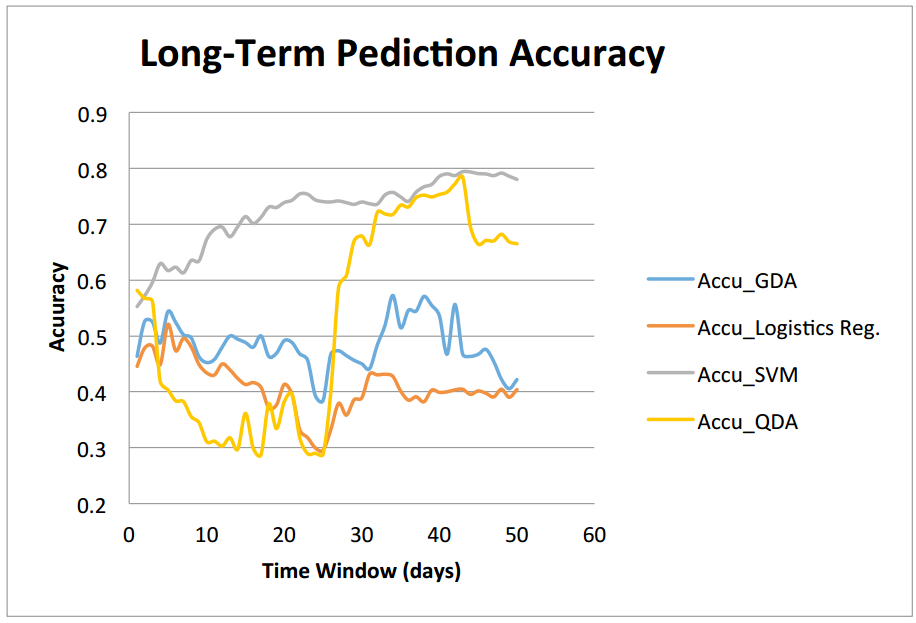
\includegraphics[height=3.5in, keepaspectratio=true]{longtermmodel.png}
\caption{Đồ thị đánh giá mô hình Dài hạn}
\end{figure}\\
Hai mô hình với hai kết quả, ta thấy ở mô hình Dài hạn hai giải thuật SVM và 
QDA cho kết quả Accuracy gần bằng 80\% với $n=44$ ngày, so sánh với mô hình 
Ngày tiếp theo Accuracy gần bằng 60\% ta có thể thấy mô hình dài hạn cho kết 
quả có ý nghĩa hơn. Nhưng một hạn chế rất lớn của công trình này, nhóm tác giả 
chỉ sử dụng một tham số đánh giá duy nhất là Accuracy mà bỏ qua Precision và 
Recall. Việc đánh giá chỉ dựa trên duy nhất một tham số sẽ không thể tổng quát 
được kết quả đầu ra, vì vậy mà dẫn đến nguy cơ không phát hiện các vấn đề về 
lệch dữ liệu hoặc overfitting.\\\\ 
Tổng quan qua hai công trình và tham khảo một số công trình khác, nhận thấy 
đa số các hướng tiếp cận đều đi theo một phương pháp tổng quát chung, nó bao gồm các bước 
cơ bản như:
\begin{enumerate}
\item Xây dựng không gian vector thuộc tính phù hợp với tính chất bài toán
\item Sử dụng các giải thuật phân lớp điển hình trong Máy học như là 
SVM, LR ...
\item Đánh giá giải thuật bằng các tham số Accuracy, Recall, Precision.
\end{enumerate}
Từ những đục kết trên, bản thân nhận thấy các bước trên cũng chính là phương pháp 
nên dùng để tiếp cận đề tài. Ngoài ra, nhận thấy ở hai công trình trên chưa 
hề sử dụng một giải thuật rất được phổ biến hiện nay, nó nổi lên như một đại 
diện của Học sâu - Deep Learning đó là MNN. Do đó mà luận văn này sẽ sử dụng 
MNN như là một giải thuật bổ sung trong quá trình so sánh và đánh giá so với 
các giải thuật phân lớp khác. 
%====================== Ly thuyet ==================
\chapter{Nền tảng lý thuyết}
\section{Bitcoin}
Các hình thức thương mại trên Internet ngày này hầu như đều dựa vào một tổ chức 
bên thứ ba đáng tin cậy để xử lý các hoạt động thanh toán điện tử. Tuy rằng sau 
nhiều năm phát triển, các tổ chức bên thứ ba này đều đã nâng cao mức độ tin cậy, 
an toàn nhưng đa số vẫn còn tồn tại những điểm yếu: không thể tránh khỏi những 
tranh chấp, phí trung gian, đòi hòi phải cung cấp các thông tin cá nhân... Và 
Bitcoin - hệ thống tiền điện tử ngang hàng (A Peer-to-Peer Electronic Cash System) 
được sinh ra để giải quyết các vấn đề trên \cite{BitcoinPaper}.
\subsection{Máy chủ nhãn thời gian - Timestamp Server}
Máy chủ nhãn thời gian hoạt động bằng cách lấy giá trị băm của block liền trước 
và thông tin của block hiện tại, cho qua hàm băm để được một giá trị băm mới. 
Giá trị băm sau khi được tính toán sẽ được công bố rộng rãi và giá trị băm này 
chứng minh rằng block tồn tại, các block được nối với nhau thành một chuỗi xác 
định.\\
\begin{figure}[h!]
\centering
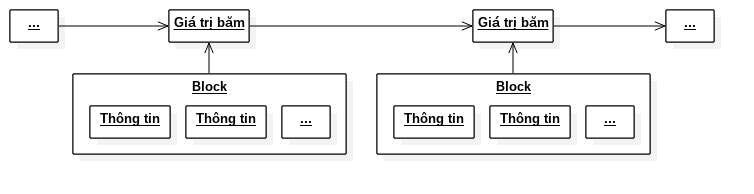
\includegraphics[height=1.45in, keepaspectratio=true]{timestampserver.png}
\caption{Máy chủ nhãn thời gian}
\end{figure}\\
\subsection{Giao dịch - Transaction (trên Blockchain)}
Bitcoin tổ chức các giao dịch bằng cách xây dựng một chuỗi các chữ ký số. Một 
địa chỉ có chứa một lượng BTC được gọi là một chủ sở hữu, một chủ sở hữu 
chuyển một lượng BTC cho một chủ sở hữu khác - người thụ hưởng - bằng cách ký 
lên giá trị băm (hash), trong đó giá trị băm là kết quả sau khi đi qua hàm băm
của tổ hợp giá trị băm giao dịch trước với địa chỉ người thụ hưởng.\\
\begin{figure}[h!]
\centering
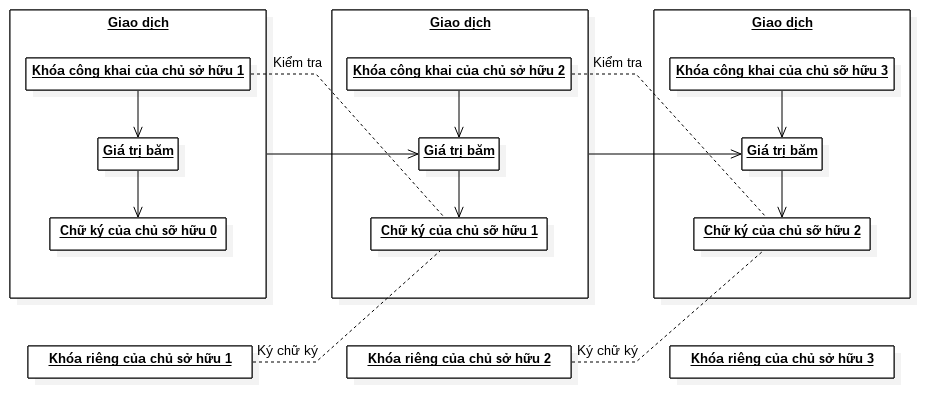
\includegraphics[height=2.45in, keepaspectratio=true]{transaction.png}
\caption{Giao dịch}
\end{figure}\\
\subsection{Proof-of-Work}
Proof-of-Work được hiểu là bằng chứng để chứng minh quá trình lao động, nó dùng 
để kiểm tra quá trình tạo ra kết quả hợp lệ là một quá trình ``lao động'' có 
sử dụng và tiêu tốn tài nguyên.\\\\
Proof-of-Work được sử dụng trong Bitcoin có cơ chế dựa trên hàm băm, ví dụ như 
SHA-256. Quá trình proof-of-work là quá trình đi tăng một con số - gọi là số 
$nonce$ - sao cho giá trị băm của số $nonce$ này cho kết quả đầu ra phải thỏa 
mãn tồn tại $n$ bit 0 ở vị trí đầu, với $n$ xác định và được gọi là số bit 0 
yêu cầu.
\subsection{Blockchain}
Blockchain được hình thành dựa trên sự kết hợp giữa máy chủ nhãn thời gian và 
proof-of-work. Blockchain là một chuỗi các block được kết nối một cách luận lý 
với nhau thông qua các mỗi quan hệ toán học và mật mã, các quan hệ này đảm bảo 
cho hệ thống luôn đúng đắn, không thể sửa và dễ dàng để kiểm tra. Block mới được 
sinh ra phải dựa trên quá trình proof-of-work.\\\\
Quá trình hình thành blockchain được bắt đầu bằng proof-of-work, các peer sẽ đi
tìm số $nonce$ sao cho sau khi cho qua hàm băm kết quả đạt được là một giá trị 
băm thỏa mãn số bit 0 yêu cầu. Số $nonce$ vừa được tìm ra sẽ được đưa và block
mới cùng với các thông tin khác như: thông tin các giao dịch, giá trị băm của 
block kề trước... Tiếp tục như vậy, các block mới được sinh ra và được kết nối 
với block cuối cùng của chuỗi.\\
\begin{figure}[h!]
\centering
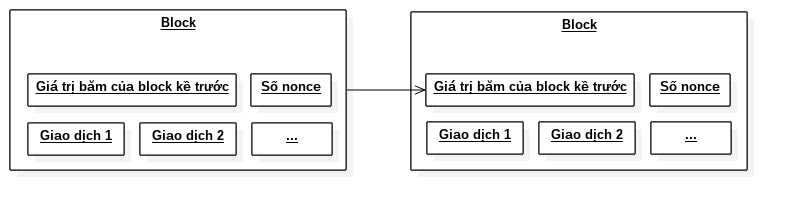
\includegraphics[height=1.5in, keepaspectratio=true]{blockchain.png}
\caption{Blockchain}
\end{figure}\\
Vì hệ thống có tính phân tán nên trên toàn mạng sẽ có nhiều phiên bản của blockchain,
cũng chính vì thế để giải quyết tính đồng nhất, chỉ blockchain có độ dài lớn 
nhất mới được xem là blockchain hợp lệ. Đồng thời để kiểm soát được tốc độ sinh
block mới, hệ thống sẽ quy định một độ khó, nếu toàn mạng có tốc độ sinh block 
(số block được sinh ra trong một giờ đồng hồ) cao hơn mức quy định, độ khó sẽ tăng lên 
để điều chỉnh lại tốc độ của toàn mạng.
\subsection{Mạng - Network}
Mỗi thành viên (máy tính, phần cứng ASIC, thiết bị di dộng... ) khi tham gia vào quá 
trình tính toán của toàn mạng thì sẽ được xem như một node. Toàn mạng sẽ hiện thực hệ 
thống bằng cách thực hiện các bước như sau:
\begin{enumerate}
\item Một gia dịch mới được truyền đi cho tất cả các node (broadcast).
\item Mỗi node sẽ lựa chọn và thu thập các giao dịch để đưa vào block.
\item Mỗi node sẽ thực hiện proof-of-work, tìm ra số $nonce$.
\item Khi một node hoàn thành proof-of-work, node này sẽ đóng block và truyền 
đi toàn tất cả các node khác.
\item Các node khác sẽ kiểm tra thông tin của block nhận được (thông tin các 
transaction, thông tin proof-of-work...) và chấp nhận block này nếu tất cả 
các thông tin đều được kiểm tra chính xác.
\item Các node sẽ thể hiện sự chấp nhận của mình bằng cách thực hiện proof-of-work 
để sinh ra block mới block này sẽ được gắn vào liền sau block mà node đã chấp nhận 
(thêm giá trị băm của block trước mà node chấp nhận vào trong block mới sinh ra).
\end{enumerate}
Lưu ý, một giao dịch mới không nhất thiết phải được truyền đến tất cả các node. 
Chỉ cần việc truyền đến số node đủ nhiều để đảm bảo việc sẽ được đưa vào một block 
và được đóng trong blockchain với độ dài lớn nhất. Cũng như vậy đối với block, 
block không nhất thiết phải được truyền đến tất cả các node, khi một node nhận 
được một block kế block bị thiếu, bằng quá trình kiểm tra node có thể biết được 
và yêu cầu các node khác trong mạng gửi cho node này block bị thiếu sót.
\subsection{Phần thưởng khích lệ}
Trong tập các giao dịch được đóng trong một block sẽ luôn tồn tại một giao dịch 
đặc biệt, giao dịch khác với các giao dịch bình thường, nó không có người chủ 
sở hữu mà chỉ có người thụ hưởng. Điều này giải thích cách mà BTC mới được sinh 
ra, cứ mỗi block được tìm ra nhờ quá trình proof-of-work sẽ có một lượng BTC 
được sinh ra và chính là phần thưởng cho người tạo ra block, điều này đồng nghĩa 
địa chỉ người thụ hưởng chính là địa chỉ của người tạo ra block.\\\\
Ngoài ra, phần thưởng khích lệ khi tạo ra được một block còn bao gồm cả phí giao 
dịch từ các giao dịch đã được đóng trong block. Phí giao dịch thường rất nhỏ và
không đáng kể ở thời điểm hiện tại.
\subsection{Tổ chức lưu trữ thông tin giao dịch}
Đối với các node là các hệ thống máy tính lớn, khả năng lưu trữ và xử lý mạnh thì 
việc lưu một block với đầy đủ các thông tin không gặp nhiều vấn đề. Nhưng đối 
với các thiết bị di động hoặc các thiết bị khác với tài nguyên lưu trữ và xử lý 
tương đối hạn hẹp thì việc lưu một blockchain đầy đủ là khá khó khăn.\\\\
Cây Merkle là một cấu trúc tổ chức dữ liệu, trong đó giá trị của node cha sẽ 
là kết quả hàm băm tất cả các giá trị (nhãn hoặc dữ liệu) của nốt con. Các nốt 
không phải lá thì giá trị sẽ là nhãn - kết quả hàm băm, các nốt lá sẽ có giá trị 
là dữ liệu cần được tổ chức.\\\\
Bitcoin sử dụng cây Merkle để tổ chức các giao dịch, nốt cao nhất của cây được 
gọi là giá trị băm gốc (Root hash) và giá trị này sẽ được lưu vào block. Ở đây,
ta thấy việc thay đổi bất kỳ một giá trị nào trong cây cũng sẽ dẫn đến việc thay 
đổi giá trị băm gốc, vì thế giá trị băm gốc khi được lưu vào block nó có chức 
năng dùng để kiểm tra lại các giao dịch trong block đó là toàn vẹn hay không.\\
\begin{figure}[h!]
\centering
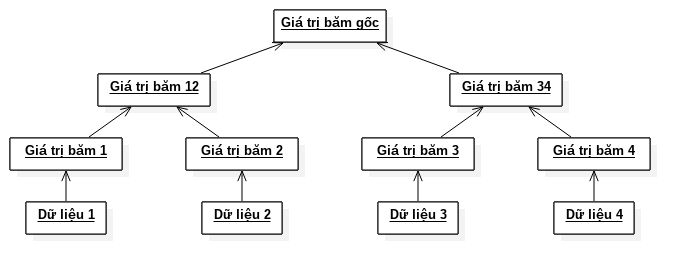
\includegraphics[height=2.25in, keepaspectratio=true]{merkletree.png}
\caption{Cây Merkle}
\end{figure}
\begin{figure}[h!]
\centering
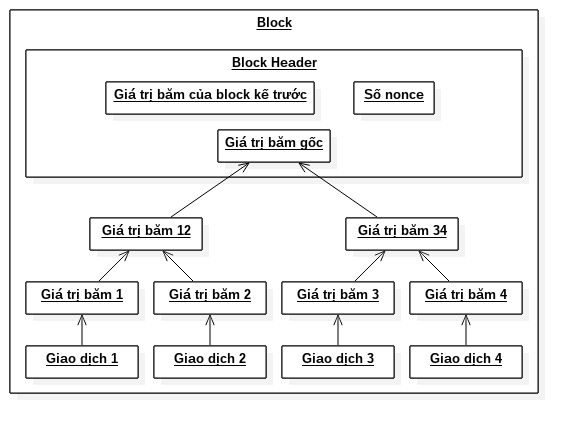
\includegraphics[height=3.75in, keepaspectratio=true]{block.png}
\caption{Cấu trúc tổ chức giao dịch trong một block}
\end{figure}\\
Một node với tài nguyên hạn chế khi muốn lưu blockchain không nhất thiết phải 
lưu đầy đủ thông tin của từng block trong blockchain, thay vào đó node có thể 
lược bỏ các thông tin về giao dịch được đóng trong block và chỉ lưu giá trị băm 
gốc của các giao dịch này. Điều này làm giảm chi phí về lưu trữ nhưng vẫn đảm 
bảo được tính toàn vẹn, khi muốn xác minh bất kỳ giao dịch nào, node chỉ cần 
yêu cầu các giao dịch trong block và tính toán lại giá trị băm gốc, nếu giá trị 
băm nào giống với giá trị băm gốc được lưu nghĩa là các giao dịch hoàn toàn hợp 
lệ.
\section{Một số khái niệm về tài chính}
Vì luận văn này đang giải quyết một bài toán về kinh tế nên để hiểu được công 
việc, ta cần nắm được các ý niệm cơ bản về kinh tế.
\subsection{Phiên giao dịch và các giá trị cơ bản}
Gọi T là một mốc thời gian bất kỳ, P là khoảng thời gian được chọn là một phiên 
giao dịch. Ta có thể nói một cách đơn giản là phiên giao dịch được mở tại thời 
điểm T và được kết thúc tại thời điểm T + P.\\\\
Cụ thể, giả sử chọn mốc mở phiên là 9:00 am và phiên giao dịch có thời hạn là 
30 phút, điều đó có nghĩa là kết thúc phiên giao dịch sẽ là 9:30 am.\\\\
Ngoài ra:
\begin{itemize}
\item Giá mở phiên: là giá bán của một giao dịch gần nhất sau thời điểm T. Ví dụ tại thời 
điểm 9:01 am có một giao dịch bán 1 BTC là \$779 và trong khoảng thời gian 9:00 am 
đến 9:01 am không hề có bất kỳ giao dịch nào khác ngoại trừ giao dịch này, thì ta có thể 
nói giá mở phiên sẽ là \$779.
\item Giá đóng phiên: là giá bán của một giao dịch gần nhất trước thời điểm T + P.
\item Giá phiên cao nhất: là giá bán cao nhất của một giao dịch trong khoảng thời gian diễn ra phiên 
giao dịch, cụ thể là từ thời điểm T đến thời điểm T + P. Ví dụ, trong khoảng thời gian 9:00 am (thời điểm 
mở phiên) đến thời gian 9:30 am (thời điểm đóng phiên) có một giao dịch BTC với giá là 
\$801 và là giao dịch có giá trị cao nhất. Vậy ta có thể nó giá phiên cao nhất là 
\$801.
\item Giá phiên thấp nhất: là giá bán thấp nhất của một giao dịch trong khoảng thời gian diễn ra phiên 
giao dịch, cụ thể là từ thời điểm T đến thời điểm T + P.
\item Lượng giao dịch: tổng giá trị USD được dùng để  mua/bán BTC trong một phiên giao dịch.
\item Trung bình giao dịch: giá trị USD trung bình của tất cả các giao dịch diễn 
ra trong khoảng thời gian một phiên giao dịch.
\end{itemize}
\subsection{Rate of Change}
Đại lượng đo sự khác nhau của giá tại phiên thứ x so với n phiên trước đó. 
Giá sử $P(x)$ là giá của phiên thứ $x$ thì:
\[ ROC_{n}(x)=\frac{P(x)-P(x-n)}{P(x-n)}\]
Nếu $ROC > 0$ thì giá thị trường đang có xu hướng đi lên (tăng giá).
Ngược lại, với $ROC < 0$ thì giá thị trường đang có xu hướng giảm xuống.
\subsection{Stochastic Oscillator}
Đại lượng dùng để đo xu hướng mua/bán của thị trường tại thời điểm phiên x thông 
qua n phiên trước đó. Giả sử:\\\\
\tab $L_{n} = $ giá phiên thấp nhất trong n phiên\\
\tab $H_{n} = $ giá phiên cao nhất trong n phiên\\
\tab $P(x) = $ giá của ngày x\\
\[\%K=\frac{P(x)-L_{n}}{H_{n}-L_{n}}\]
Nếu $ \%K $ nhỏ hơn 20 thì thị trường đang có xu hướng mua vào và nếu lớn hơn 
80 thì thị trường đang có xu hướng bán ra.


\section{Máy học}

\subsection{Khái niệm cơ bản}
\subsubsection{Máy học}
Máy học có hai cách định nghĩa chính và đang được chấp nhận phổ biến:
\begin{itemize}
  \item Theo Arthur Samuel: \textit{``Là một lĩnh vực nghiên cứu mà nó cung cấp cho
  máy tính khả năng học hỏi mà không cần lập trình một cách tường minh.''}
  \item Theo Tom Mitchell: \textit{``Một chương trình máy tính được chấp nhận
  là học hỏi được kinh nghiệm E bằng cách thực hiện một vài tác vụ T theo phép đo hiệu
  năng P, nếu và chỉ nếu việc thực thi các tác vụ trong T được đo bởi phép đo P
  đem lại kết quả là kinh nghiệm E được cải thiện.''}
\end{itemize}
\subsubsection{Supervised Learning - Học có giám sát}
Chúng ta được cho một tập dữ liệu đã biết với các input và output tương ứng
nhau. Ý tưởng là chúng ta sẽ đi tìm mối quan hệ giữa input và output đó chính là
Supervised Learning.\\\\
Vấn đề của Supervised Learning được phân loại thành hai
vấn đề chính là “Regression” và “Classification”. Trong vấn đề “Regression”,
chúng ta sẽ cố gắng dự đoán kết quả output tiếp theo một cách liên tục, nghĩa là
chúng ta đi tìm ra một hàm đầu ra liên tục tổng quát với biến là các thuộc tính
đầu vào. Còn với vấn đề “Classification”, chúng ta thay vì cố gắng dự đoán kết
quả liên tục thì ta sẽ đi dự đoán chúng theo hướng rời rạc, hiểu theo một cách
khác là chúng ta đi tìm một phép phân loại rời rạc cho output với các biến
input.
\subsubsection{Unsupervised Learning - Học không giám sát}
Học không giám sát cho phép chúng ta tiếp cận các vấn đề mà ta chưa hề hoặc biết
rất ít kết quả của chúng ta sẽ trông như thế nào. Chúng ta có thể xây dựng cấu
trúc của dữ liệu mà không cần thiết phải biết ảnh hưởng của các biến đó.\\\\
Chúng ta thực hiện việc này dựa trên ý tưởng gom cụm dữ liệu bằng cách xem xét
mối quan hệ giữa các thuộc tính của dữ liệu. Các hướng tiếp cận dựa trên nhưng 
phương pháp như vậy thường được gọi là “Clustering”.

\subsection{Thông số đánh giá}
Có ba tham số cơ bản dùng để xem xét và đánh giá giải thuật trong Máy học.
Gọi:
\begin{itemize}
\item True positive là TP
\item False positive là FP
\item True negative là TN
\item False negative là FN
\end{itemize}
Thì:\\
\[
  Accuracy = \frac{TP+TN}{TP+FP+TN+FN}
\]
\[
  Precision = \frac{TP}{TP+FP}
\]
\[
  Recall = \frac{TP}{TP+FN}
\]\\
\begin{figure}[h!]
\centering
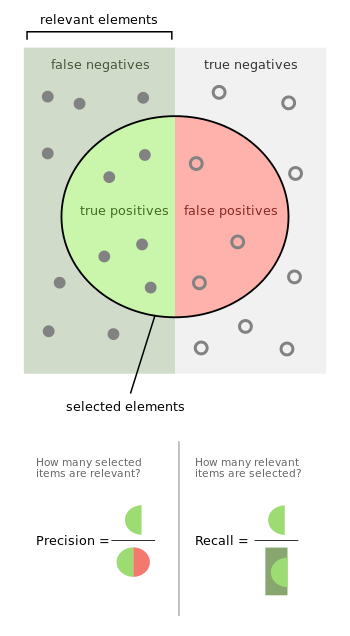
\includegraphics[height=7in, keepaspectratio=true]{precision_recall.png}
\caption{Validation Parameters}
\end{figure}\\
\subsection{Neural Network - Deep Learning}
Deep Learning nói chung và Neural Network nói riêng là hai phạm trù xuất hiện 
không lâu đối với Máy học, đại diện cho hướng tiếp cận gần với 
cái nhìn thực tế, học nhiều cấp và học từ bản chất dữ liệu. Deep Learning 
thường giải quyết rất tốt với các loại dữ liệu mang tính ``con người'' như 
hình ảnh, âm thanh ... \cite{NeuralNetworksandDeepLearning} 
\subsubsection{Ý tưởng giải thuật}
Bộ não con người là một trong những phát minh vĩ đại nhất của tự nhiên, nó 
có thể giải quyết các bài toán mà đối với máy tính là cực kỳ phức tạp chỉ trong 
vài giây hoặc kể cả là vài phần giây, các khả năng phán đoán, học hỏi, tích lũy 
kinh nghiệm đó chính là điều tuyệt diệu của bộ não con người. Và các nhà khoa học 
khao khát một thứ gì đó trong giới máy tính có khả năng như vậy.\\\\
Dựa trên ý tưởng kết cấu của bộ não gồm hàng tỷ neural liên kết lại với nhau, 
mỗi neural chỉ đưa ra một tín hiệu hết sức đơn giản, nhưng khi hàng tỷ neural liên kết 
hình thành nên một hệ thống phức tạp thì từ đó có khả năng giải quyết các vấn đề 
phức tạp. Các nhà khoa học máy tính, đã cố gắng định nghĩa một neural đơn lẻ 
trong phạm trù máy tính và được gọi là perceptron, từ đó kết nối lại với nhau 
để tạo nên một hệ thống hữu hạn các perceptron có khả năng giả lập một bộ não 
người - mạng neural nhân tạo.

\subsubsection{Cấu trúc một Perceptron}
Một perceptron sẽ có các input $x_1, x_2, ...$ và output sẽ là một giá trị 
nhị phân.\\
\begin{figure}[h!]
\centering
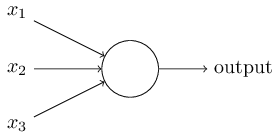
\includegraphics[height=1.5in, keepaspectratio=true]{perceptron.png}
\caption{Perceptron}
\end{figure}\\
Một ví dụ đơn giản dựa vào hình trên, ta thấy perceptron này có 3 input là 
$x_1, x_2, x_3$ , giả sử đi kèm với mỗi input sẽ có một giá trị trọng 
số $w_1, w_2, w_3$. Output được định nghĩa là 0 và 1, nhận giá trị 0 
khi $\sum_j w_j x_j$ nhỏ hơn giá trị ngưỡng và 1 khi lớn gơn giá trị ngưỡng.\\\\
Biểu diễn đại số:\\
\[
  output = 
  \bigg\{
    _{0 \quad if \, \sum_j w_j x_j \, \leq \, threshold}
    ^{1 \quad if \, \sum_j w_j x_j \, > \, threshold}
\]
Các hàm số như trên được gọi là activation function, có nhiều loại activation
 function khác nhau như: $sigmoid , tang ...$ 

\subsubsection{Multilayer Neural Network}
Hiển nhiên, một perceptron không thể mô phỏng nên được một bộ não người, để 
có thể đưa ra một quyết định tương tự như bộ não người các perceptron này cần 
được kết nối với nhau thành một mạng lưới - Multilayer Neural Network.\\
\begin{figure}[h!]
\centering
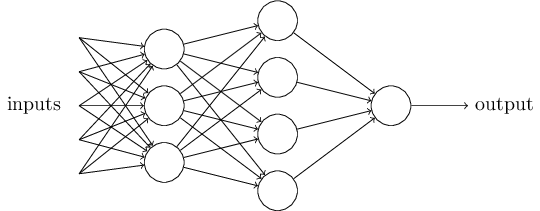
\includegraphics[height=2in, keepaspectratio=true]{multilayerneuralnetwork.png}
\caption{Multilayer Neural Network}
\end{figure}\\
Multilayer Neural Network được cấu thành bằng cách sắp xếp các perceptron thành 
từng lớp. Các perceptron ở mỗi lớp sẽ kết nối với tất cả các perceptron ở các 
lớp liền kề, cột những perceptron đầu tiên được gọi là input layer, chúng có 
chức năng tiếp nhận các input để cho ra các output. Các output ở lớp trước sẽ chính là 
input cho các perceptron ở lớp tiếp theo. Các perceptron ở lớp cuối cùng được gọi là 
output layer, trong trường hợp này đặc biệt chỉ có duy nhất một perceptron. Còn 
lại các lớp perceptron khác được gọi là hidden layer.\\\\
Giả sử input của perceptron là $x_1, x_2, ...$ tương ứng là đó là các trọng 
số $w_1, w_2, ...$. Thêm vào đó định nghĩa về bias, ở đây bias là một giá trị 
đại diện độ lệch của từng perceptron và được ký hiệu $b_1, b_2, ...$. Ta có biểu diễn của activation 
function:\\
\[
  output = 
  \bigg\{
    _{0 \quad if \, \sum_j w_j x_j + b_i\, \leq \, 0}
    ^{1 \quad if \, \sum_j w_j x_j + b_i\, > \, 1}
\]
Ví dụ:\\
\begin{figure}[h!]
\centering
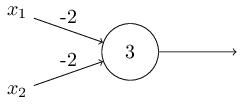
\includegraphics[height=1in, keepaspectratio=true]{exmln.png}
\caption{Perceptron with Bias example}
\end{figure}\\
Ta có $w_1=w_2=-2$ và $b=3$, khi đó nếu input $x_1=1,\, x_2=0$ suy ra $ 
w_1*x_1+w_2*x_2+b=(-2)*1+(-2)*0+3=1$, ta có thể chọn $threshold=0$ vì $1>0$
nên $output=1$.

\subsubsection{Sigmoid Function - Hàm Sigmoid}
Với dạng activation function được định nghĩa ở trên, giá trị của activation 
function gần như không có giới hạn. Vậy tại sao việc không có giới hạn lại 
cần được quan tâm. Trong một trường hợp cụ thể, với việc sử dụng activation 
function như trên có thể dẫn đến trường hợp đầu ra của một perceptron sẽ nhận 
giá trị rất lớn - giả sử là 1000, những một perceptron khác sẽ nhận giá trị rất 
bé - giả sử 0.001. Vì thế khi đến lớp tiếp theo thì gần như perceptron cho kết 
quả đầu ra là giá trị bé sẽ mất đi độ ảnh hưởng và làm mất cân đối cho toàn mạng.\\\\
Do đó để giới hạn giá trị của activation function chúng ta sẽ sử dụng hàm sigmoid. 
Sigmoid function được định nghĩa như sau:\\
\[
  \sigma(z)=\frac{1}{1+e^{-z}}
\]
Áp dụng Sigmoid function vào activation function ta có activation function dạng
sigmoid và khi đó activation function của chúng ta sẽ có dạng:\\
\[
  \frac{1}{1+exp(-\sum_j w_j x_j -b)}
\]
Lúc này ta có một activation function có giá trị được giới hạn trong khoảng 
từ 0 đến 1. Nhưng chú ý, giá trị của activation function là liên tục, để rời 
rạc hóa giá trị của activation function ta có thể sử dụng một phương pháp 
quen thuộc - sử dụng threshold. Điển hình ta chọn threshold = 0.5, nếu lớn hơn 
thì activation function sẽ nhận 1 và ngược lại sẽ nhận 0.\\\\
Để hiểu rõ hơn tại sao chúng ta quan sát hai đồ thị của sigmoid function và 
activation function có dạng sigmoid và đã được rời rạc hóa giá trị:\\
\begin{figure}[h!]
\centering
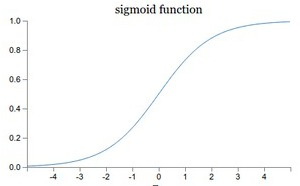
\includegraphics[height=2.5in, keepaspectratio=true]{sigmoid.jpg}
\caption{Sigmoid Function}
\end{figure}\\
\begin{figure}[h!]
\centering
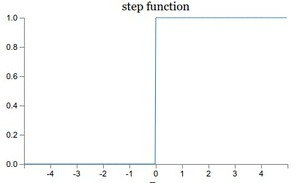
\includegraphics[height=2.5in, keepaspectratio=true]{step.jpg}
\caption{Step Function}
\end{figure}\\

\subsubsection{Giải thuật Backpropagation}
Sau khi đã có xây dựng thành công một mô hình Multilayer Neural Network, công 
việc cuối cùng là cung cấp khả năng tự học hỏi từ đó để bản thân mạng có thể 
tự xây dựng mô hình và đưa ra các quyết định cụ thể.\\\\
Cụ thể, khi nhìn lại một Multilayer Neural Network với activation function là 
sigmoid function thì các tham sô $w, b$ là chưa biết và việc cung cấp khả năng 
tự học hỏi chính là cung cấp một giải thuật giúp mạng tìm được các tham số 
$w, b$ với một tập kinh nghiệm - hay tập huấn luyện - ${x, y}$ cụ thể, trong 
đó $x$ là input và $y$ là output tương ứng với từng bộ $x$. Giải thuật backpropagation 
là một trong nhưng giải thuật chúng ta cần tìm.\\\\
Trước tiên chúng ta cần đi qua một số ký hiệu:\\\\
\begin{itemize}
\item $w$ là vector của các giá trị trọng số\\ 
\[ w =
\begin{bmatrix}
w_1\\
\vdots\\
w_n
\end{bmatrix}
\]
\item $b$ là vector của các giá trị bias\\ 
\[ b =
\begin{bmatrix}
b_1\\
\vdots\\
b_m
\end{bmatrix}
\]
\item $\sigma$ là sigmoid function
\item $a(\sigma)$ là activation function có dạng sigmoid
\end{itemize}
Biểu diễn activation function:\\
\begin{figure}[h!]
\centering
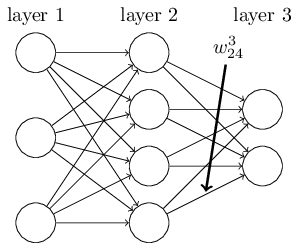
\includegraphics[height=2in, keepaspectratio=true]{exw.png}
\caption{Weight Notation example}
\end{figure}\\
Ví dụ như hình trên, trọng số xuất phát từ perceptron thứ 4 thuộc layer thứ 
2 và kết thúc tại perceptron thứ 2 thuộc layer thứ 3 được ký hiệu là 
$w_{24}^3$.\\\\
Tương tự như vậy với bias và activation function của perceptron thứ j thuộc layer 
thứ l của mạng sẽ được kí hiệu thứ tự là $b_j^l,\,a_j^l$. Ví dụ, bias của perceptron 
thứ 3 thuộc layer thứ 2 sẽ là $b_3^2$ và activation function của perceptron thứ 
1 thuộc layer thứ 3 sẽ là $a_1^3$.\\
\begin{figure}[h!]
\centering
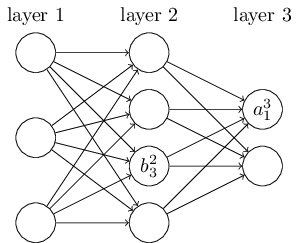
\includegraphics[height=2in, keepaspectratio=true]{exb.png}
\caption{Bias Notation example}
\end{figure}\\
Lúc này ta có biểu diễn toán học đầy đủ của activation function:\\
\[
  a_j^l=\sigma(\sum_k w_{jk}^l a_k^l-1 + b_j^l)
\]
Với ký hiệu vector ta có thể tổng quát phát biểu với dạng:\\
\[
  a^l=\sigma(w^l a^{l-1} + b^l)
\]
\textbf{Cost function:} Trước khi đi vào hiểu được backpropagation có thể làm gì, 
chúng ta cần phải biết một định nghĩa cost function. Vậy cost function là gì? 
Đúng theo tên của hàm, nó dùng để đo lường chi phí của thuật toán. Chi tiết:\\
\[
  C=\frac{1}{2n}\sum_x\|y(x)-a^L(x)\|^2
\]
Ta có thể thấy, dạng hàm số trên hết sức quen thuộc với định nghĩa độ lệch chuẩn 
trong xác suất thống kê nhưng đã được biến đổi một chút. Thay vì giá trị kỳ vọng 
và các điểm xác suất, cost function sử dụng giá trị thực tế $y$ của tập dữ liệu 
và giá trị $y=a$ là giá trị $y$ tính toán được từ $x$ với $w$ và $b$. Vậy ta 
có thể hiểu được, cost function tính toán độ sai lệch của giá trị $a$ so với 
$y$ kỳ vọng thực tế. Do đó, cost function càng nhỏ thì biểu diễn giá trị của 
Multilayer Neural Network sẽ càng gần với thực tế.\\\\
Để tìm được giá trị cực tiểu cho cost function ta sẽ thực hiện vòng lặp:\\
\[
  w_ij^{(l)}:=w_ij^{(l)}-\eta\frac{\sigma}{\sigma w_ij^{(l)}}C(w,b)
\]
\[
  b_i^{(l)}:=b_i^{(l)}-\eta\frac{\sigma}{\sigma b_i^{(l)}}C(w,b)
\]

Trong đó $\eta$ là learning rate - tỉ lệ học, việc hội tụ về giá trị cực tiểu với 
tốc độ và độ chính xác phụ thuộc vào tỉ lệ này.\\\\
Vậy, đi qua một quá trình tìm hiểu về Multilayer Neural Network, ta có thể hiểu 
được việc học hỏi kinh nghiệm của mạng cốt lõi vẫn là việc tìm ra bộ $w$ và $b$ 
tương ứng với ${x, y}$ của bộ dữ liệu luyện tập, và để tìm ra được $w$ và $b$ 
ta có thể sử dụng giải thuật backpropagation.
\chapter{Các giải thuật gom cụm}
\section{Giải thuật K-Means}
Vì giải thuật K-means khá đơn giản và có thể hữu hình hóa nên chúng ta sẽ đi
thẳng vào thuật toán để xem các bước thực hiện của giải thuật K-means như thế
nào, từ đó ta cũng có thể hiểu được cách tiếp cận vấn đề của giải
thuật.\\\\ 
 Các bước của giải thuật K-means được thực hiện theo trình tự:
\begin{enumerate}
  \item Gọi k là số cụm mong muốn, bắt đầu với việc chọn ngẫu nhiên các
  vector ``trọng tâm'' của k nhóm $\mu_1,\mu_2,\dots, \mu_k \in \mathbb{R} ^n $.
  \item Lặp cho đến khi hội tụ: \{ \\\\
  Với mỗi i, tính:
  \[ c^{(i)} := arg\:min_j||x^{(i)} - \mu_j||^2 \]
  Với mỗi j, tính:
  \[ \mu_j
  :=\frac{\sum_{i=1}^{m}1\{c^{(i)}=j\}x^{(i)}}{\sum_{i=1}^{m}1\{c^{(i)}=j\}}
  \]
  \}\\\\
  Dưới đây là hình mô phỏng cách thuật toán làm việc, với ví dụ điển hình là
  vector 2 chiều (Hình ảnh được trích từ CS229 Lecture Notes – 7a. The k-means
  clustering algorithm – Andrew Ng):\\\\\\\\\\\\
  \begin{figure}[h!]
  	\centering
	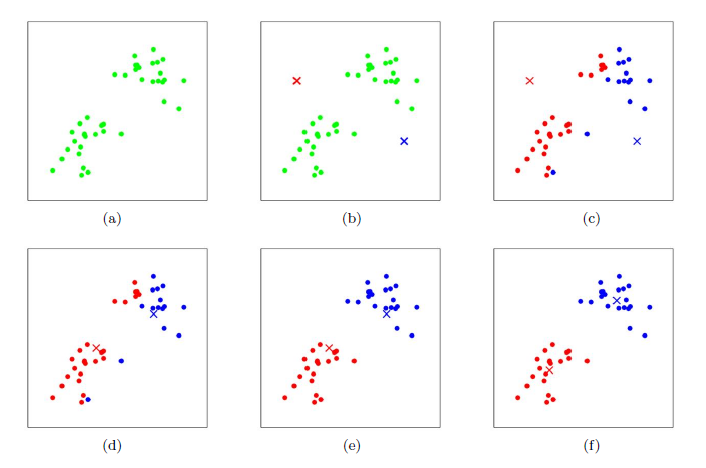
\includegraphics[width=7in,height=3in,keepaspectratio=true]{kmeans.png}
	\caption{Thuật toán K-means với vector 2 chiều}
  \end{figure}
  
  Giải thích hình trên:
  \begin{enumerate}
    \item Ta có tập dữ liệu đầu vào không nhãn, ta muốn chia tập dữ liệu
    này thành hai cụm.
    \item Ta chọn hai vector “trọng tâm” ban đầu bất kỳ, mỗi vector đại diện cho
    một cụm và được biễu diễn bằng điểm x trên đồ thị. Đây chính là bước (a) của thuật toán.
    \item Ở đây, ta giả sử vector “trọng tâm” nằm góc trên bên phải có giá trị
    $\mu_1$ đại diện cho nhãn $\{c^{(i)}=1\}$ và vector “trọng tâm” nằm góc dưới
    bên phải có giá trị $\mu_2$ đại diện cho nhãn $\{c^{(i)}=2\}$. Bắt đầu vào
    vòng lặp đầu tiên của bước (b). Thuật toán đi tính khoảng cách Euclid của
    tất cả các vector phần tử trong tập dữ liệu đến hai vector “trọng tâm”. Phần
    tử được đánh nhãn $\{c^{(i)}=1\}$ khi khoảng cách Euclid đến vector “trọng
    tâm” $\mu_1$ gần hơn so với vector “trọng tâm” $\mu_2$ hoặc ngược lại. Cứ
    tiếp tục như vậy ta sẽ gán nhãn cho tất cả các phần tử trong tập dữ liệu đầu vào.
    \item Ta cập nhật lại giá trị của vector “trọng tâm” bằng cách gán
    $\mu_j(j=1 \vee 2)$ bằng với giá trị trung bình của các phần tử thuộc nhãn
    do chính nó sở hữu. Đây chính là vòng lặp thứ 2 trong bước (b).
    \item Ta quay lại từ đầu của bước (b).
    \item Tiếp tục cập nhật cho đến khi hội tụ.
  \end{enumerate}
\end{enumerate}
\section{Giải thuật kết hợp Gaussian và EM (Mixture of Gaussians and
the EM Algorithm)}
Để giải quyết bài toán phân cụm, ta sẽ tiếp cận với một giải thuật dựa trên
nguyên lý của phân phối Gaussian và thuật toán EM – Expectation
Maximization.\\\\ 
Giả sử ta có bộ dữ liệu đầu vào được biểu diễn dưới dạng
$\{x^{(1)},\dots,x^{(m)}\}$, yêu cầu của bài toán là đưa ra kết quả với mỗi phần
tử trong tập dữ liệu được phân thành các cụm với các phần tử khác có “tính chất
tương tự nhau”. Lưu ý, tập dữ liệu của chúng ta không tồn tại nhãn.\\\\ 
Bắt đầu với “động lực” ban đầu của giải thuật, ta mong muốn chia tập dữ liệu
thành k nhóm và mỗi nhóm được đại diện bởi một mô hình phân phối xác suất. Ở
đây, nhận thấy mô hình phân phối Gaussian là thích hợp, vì giới hạn của báo cáo,
chúng ta sẽ khoan xem xét đến việc tại sao mô hình phân phối Gaussian được chọn?
Và nó thích hợp như thế nào? Mà thay vào đó sẽ đi làm rõ cách mà mô hình phân
hình Gaussian tham số hóa cho từng cụm dữ liệu của ta.\\\\ 
Xét xác suất $p(x^{(i)},z^{(i)}) = p(x^{(i)}|z^{(i)})p(z^{(i)})$. Trong công
thức này ta có $p(x^{(i)}|z^{(i)})$ là xác suất để phần tử $x^{(i)}$ thuộc vào
cụm được đánh nhãn $z^{(i)}$ và $p(z^{(i)})$ là xác suất để cụm được gán nhãn
$z^{(i)}$.\\\\ 
Từ cách giải thích đó, ta có được  $z^{(i)} \sim Multinomial(\phi
)$ (Multinominal – Phân phối đa thức) với $p(z^{(i)}=j)=\phi_j \geq 0,\:
\sum_{j-1}^{k}\phi_j =1$, và $(x^{(i)}|z^{(i)} =j)\sim
\mathcal{N}(\mu_j,\Sigma_j)$.\\\\ 
Mặc khác, như đã nó bên trên, vì $(x^{(i)}|z^{(i)} =j)\sim
\mathcal{N}(\mu_j,\Sigma_j)$ nên ta có thể viết lại xác suất ban đầu dưới dạng
phụ thuộc vào $\mu_j,\:\Sigma_j$:
\[ p(x^{(i)},z^{(i)}) = p(x^{(i)};\:\phi,\:\mu,\:\Sigma) \]
Tiếp tục phân tích:
\[ p(x^{(i)};\:\phi,\:\mu,\:\Sigma) = \sum_{z^{(i)}=1}^{k}
p(x^{(i)}|z^{(i)};\:\mu,\:\Sigma)p(z^{(i)};\:\phi) \] 
Tại đây ta thấy được bài toán thực sự được sử dụng Mixtures of Gaussian như thế
nào vào việc mô hình hóa.\\\\
Công việc tiếp theo chúng ta sẽ đi cực đại giá trị xác suất
$p(x^{(i)};\:\phi,\:\mu,\:\Sigma)$ cho từng cụm – vì ta giả sử có k cụm nên việc này đồng nghĩa ta phải cực đại cho k xác suất như
vậy. Việc này cũng có ý nghĩa là, khi ta xét một phần tử bất kỳ ta sẽ đi tính
xác suất của điểm này cho k cụm, nghĩa là thử nó với từng mô hình xác suất, và
nó sẽ được kết luận thuộc cụm có giá trị xác suất là cao nhất.\\\\ 
Để giải quyết bài toán cực đại ta sử dụng thuật toán Maximum Likelihood. Ta có
biểu thức likelihood của xác suất ban đầu với m là số phần tử của tập đầu vào:
\[ l(\phi,\:\mu,\:\Sigma) = \sum_{i=1}^{m} \log\:
p(x^{(i)};\:\phi,\:\mu,\:\Sigma) = \sum_{i=1}^{m} \log \sum_{z^{(i)}=1}^{k}
p(x^{(i)}|z^{(i)};\:\mu,\:\Sigma)p(z^{(i)};\:\phi) \]
Tạm dừng bài toán tại đây. Chúng ta sẽ chuyển sang Giải thuật EM, để cung cấp
cho chúng ta một công cụ có thể giúp tiếp tục giải quyết bài toán.\\\\ 
Định nghĩa hàm lồi – lõm: Hàm f được gọi là lồi khi $f'' \geq 0$. Ngược lại, 
$f'' \leq 0$ thì f được gọi là hàm lõm.\\\\ 
Bất đẳng thức Jensen: Cho hàm lồi f, với bất kỳ X ta luôn có:
\[ E[f(X)] \geq f[E(X)] \]
Điều kiện đẳng thức xảy ra khi $X=E[X]$\\\\
Ta có thể suy rộng ra cho trường hợp f là hàm lõm, dấu của bất đẳng thức sẽ được
đảo chiều:
\[ E[f(X)] \leq f[E(X)] \]
Điều kiện đẳng thức vẫn giữ nguyên.\\\\ 
Xét $f(x) = \log(x)$ và $x=\frac{p(x^{(i)},z^{(i)};\theta)}{Q_i(z^{(i)})} $ .
Khoan hãy nghi vấn tại sao chúng ta đặt như vậy mà hãy xem phép biến đổi dưới đây để hiểu rõ hơn:
\begin{align} \sum_{i} \log\: p(x^{(i)};\:\theta) & = \sum_{i} \log
\sum_{z^{(i)}} p(x^{(i)},z^{(i)};\:\theta) = \sum_{i} \log \sum_{z^{(i)}}
Q_i(z^{(i)})\frac{p(x^{(i)},z^{(i)};\:\theta)}{Q_i(z^{(i)})}  \notag \\
& \geq \sum_{i} \sum_{z^{(i)}}
Q_i(z^{(i)})\:\log \frac{p(x^{(i)},z^{(i)};\:\theta)}{Q_i(z^{(i)})} \notag
\end{align}
Tới đây, ta thấy được việc đặt ở trên để đưa về dạng chuẩn của bất đẳng thức
Jensen cho hàm lõm.\\\\ 
Bây giờ ta đã có đầy đủ công cụ để giải quyết tiếp bài toán ban đầu.\\\\ 
Ta đa dừng lại ở việc phải đi cực đại biểu thức Likelihood:
\[ l(\phi,\:\mu,\:\Sigma) = \sum_{i=1}^{m} \log\:
p(x^{(i)};\:\phi,\:\mu,\:\Sigma) = \sum_{i=1}^{m} \log \sum_{z^{(i)}=1}^{k}
p(x^{(i)}|z^{(i)}=j;\:\mu,\:\Sigma)p(z^{(i)=j};\:\phi) \]
Với $w_{j}^{(i)} = P(z^{(i)}=j|x^{(i)};\:phi,\:\mu,\:\Sigma)$, ta có:
\begin{multline}
\sum_{i=1}^{m} \log \sum_{z^{(i)}=1}^{k}
p(x^{(i)}|z^{(i)};\:\mu,\:\Sigma)p(z^{(i)};\:\phi) = \sum_{i=1}^{m} \log
\sum_{j=1}^{k}
w_{j}^{(i)}\frac{p(x^{(i)}|z^{(i)};\:\mu,\:\Sigma)p(z^{(i)};\:\phi)}{w_{j}^{(i)}}\\
\geq \sum_{i=1}^{m} \sum_{j=1}^{k} w_{j}^{(i)} \log
\frac{\frac{1}{(2\pi)^{n/2}|\Sigma_j|^{1/2}}\exp\left( -\frac{1}{2}
(x^{(i)}-\mu_j)^T \Sigma_j^{-1} (x^{(i)}-\mu_j)
\right).\phi_j}{w_{j}^{(i)}}\notag
\end{multline}
Để cực đại biểu thức bên phải, chúng ta thực hiện bằng cách đạo hàm từng phần
lần lượt với $\mu$, $\phi$ và $\Sigma$ sau đó đặt bằng 0, từ biểu thức thu được
ta giải nghiệm.\\\\ 
Bắt đầu với đạo hàm riêng theo $\mu_l$ với $l=1,\dots, k$
\begin{align}
\nabla_{u_l} & \sum_{i=1}^{m} \sum_{j=1}^{k} w_{j}^{(i)} \log
\frac{\frac{1}{(2\pi)^{n/2}|\Sigma_j|^{1/2}}\exp\left( -\frac{1}{2}
(x^{(i)}-\mu_j)^T \Sigma_j^{-1} (x^{(i)}-\mu_j)
\right).\phi_j}{w_{j}^{(i)}}\notag\\
& =  \nabla_{u_l} \sum_{i=1}^{m} \sum_{j=1}^{k} w_{j}^{(i)} \left( \log
\frac{\frac{1}{(2\pi)^{n/2}|\Sigma_j|^{1/2}}\phi_j }{w_{j}^{(i)}} -\frac{1}{2}
(x^{(i)}-\mu_j)^T \Sigma_j^{-1} (x^{(i)}-\mu_j) \right)\notag\\
& = \nabla_{u_l} \sum_{i=1}^{m} \sum_{j=1}^{k} w_{j}^{(i)} \log
\frac{\frac{1}{(2\pi)^{n/2}|\Sigma_j|^{1/2}}\phi_j }{w_{j}^{(i)}} -\frac{1}{2}
\nabla_{u_l} \sum_{i=1}^{m} \sum_{j=1}^{k} w_{j}^{(i)} (x^{(i)}-\mu_j)^T
\Sigma_j^{-1} (x^{(i)}-\mu_j)\notag\\
& = -\frac{1}{2} \nabla_{u_l} \sum_{i=1}^{m} \sum_{j=1}^{k} w_{j}^{(i)}
(x^{(i)}-\mu_j)^T \Sigma_j^{-1} (x^{(i)}-\mu_j)\notag\\
& = -\frac{1}{2} \sum_{i=1}^{m} \nabla_{u_l} \sum_{j=1}^{k} w_{j}^{(i)}
(x^{(i)}-\mu_j)^T \Sigma_j^{-1} (x^{(i)}-\mu_j)\notag\\
& = -\frac{1}{2} \sum_{i=1}^{m} \nabla_{u_l} w_{l}^{(i)}
(x^{(i)}-\mu_l)^T \Sigma_l^{-1} (x^{(i)}-\mu_l)\notag\\
& = -\frac{1}{2} \sum_{i=1}^{m} w_{l}^{(i)} \nabla_{u_l} 
(x^{(i)^T}-\mu_l^T) \Sigma_l^{-1} (x^{(i)}-\mu_l)\notag\\
& = -\frac{1}{2} \sum_{i=1}^{m} w_{l}^{(i)} \nabla_{u_l} (x^{(i)^T} \Sigma_l^{-1}
x^{(i)} - \mu_l^T \Sigma_l^{-1} x^{(i)} - x^{(i)^T} \Sigma_l^{-1} \mu_l + \mu_l^T
\Sigma_l^{-1} \mu_l)\notag\\
& = -\frac{1}{2} \sum_{i=1}^{m} w_{l}^{(i)} \nabla_{u_l} (- \mu_l^T \Sigma_l^{-1}
x^{(i)} - x^{(i)^T} \Sigma_l^{-1} \mu_l + \mu_l^T
\Sigma_l^{-1} \mu_l)\notag\\
& = \frac{1}{2} \sum_{i=1}^{m} w_{l}^{(i)} \nabla_{u_l} ( \mu_l^T \Sigma_l^{-1}
x^{(i)} + x^{(i)^T} \Sigma_l^{-1} \mu_l - \mu_l^T
\Sigma_l^{-1} \mu_l)\notag\\
& = \frac{1}{2} \sum_{i=1}^{m} w_{l}^{(i)} \nabla_{u_l} tr( \mu_l^T \Sigma_l^{-1}
x^{(i)} + x^{(i)^T} \Sigma_l^{-1} \mu_l - \mu_l^T
\Sigma_l^{-1} \mu_l)\notag\\
& = \frac{1}{2} \sum_{i=1}^{m} w_{l}^{(i)} \nabla_{u_l} (tr(\mu_l^T \Sigma_l^{-1}
x^{(i)}) + tr(x^{(i)^T} \Sigma_l^{-1} \mu_l) - tr(\mu_l^T
\Sigma_l^{-1} \mu_l))\notag\\
& = \frac{1}{2} \sum_{i=1}^{m} w_{l}^{(i)} \nabla_{u_l} (tr(\mu_l^T \Sigma_l^{-1}
x^{(i)}) + tr(x^{(i)^T} \Sigma_l^{-1} \mu_l)^T - tr(\mu_l^T
\Sigma_l^{-1} \mu_l))\notag\\
& = \frac{1}{2} \sum_{i=1}^{m} w_{l}^{(i)} \nabla_{u_l} (2tr(\mu_l^T \Sigma_l^{-1}
x^{(i)}) - tr(\mu_l^T \Sigma_l^{-1} \mu_l))\notag\\
& = \frac{1}{2} \sum_{i=1}^{m} w_{l}^{(i)} \nabla_{u_l} (2(\mu_l^T \Sigma_l^{-1}
x^{(i)}) - (\mu_l^T \Sigma_l^{-1} \mu_l))\notag\\
& = \sum_{i=1}^{m} w_{l}^{(i)} (\Sigma_l^{-1}
x^{(i)} - \Sigma_l^{-1} \mu_l)\notag
\end{align}
Đặt $\sum_{i=1}^{m} w_{l}^{(i)} (\Sigma_l^{-1}
x^{(i)} - \Sigma_l^{-1} \mu_l) = 0$. Giải phương trình ta được:
\[ \mu_l = \frac{\sum_{i=1}^{m} w_l^{(i)} x^{(i)}}{\sum_{i=1}^{m} w_l^{(i)}} \]
Tiếp tục với đạo hàm riêng theo $\phi_j$. Ta nhận thấy biểu thức chỉ có một biến
duy nhất phụ thuộc vào $\phi_j$ , ta dễ dàng viết được:
\begin{align} \nabla_{\phi_j} \sum_{i=1}^{m} \sum_{j=1}^{k} w_{j}^{(i)} & \log
\frac{\frac{1}{(2\pi)^{n/2}|\Sigma_j|^{1/2}}\exp\left( -\frac{1}{2}
(x^{(i)}-\mu_j)^T \Sigma_j^{-1} (x^{(i)}-\mu_j)
\right).\phi_j}{w_{j}^{(i)}}\notag\\
& =  \nabla_{\phi_j} \sum_{i=1}^{m} \sum_{j=1}^{k} w_{j}^{(i)} \log \phi_j\notag
\end{align}
Điều này đồng nghĩa với việc bài toán cực đại ban đầu theo $\phi_j$ sẽ tương ứng
với việc đi cực đại $\sum_{i=1}^{m} \sum_{j=1}^{k} w_{j}^{(i)} \log \phi_j$ theo
$\phi_j$.\\\\
Tuy nhiên, $\phi_j$ chịu ràng buộc $\sum_{j=1}^{k} \phi_j=1$ nên ta cần dùng đến
kỹ thuật Lagrangian:\\\\
Đặt:
\[ \mathcal{L}(\phi)= \sum_{i=1}^{m} \sum_{j=1}^{k} w_{j}^{(i)} \log \phi_j +
\beta \left( \sum_{j=1}^{k} \phi_j-1 \right) \]
Để cực đại $\mathcal{L}(\phi)$ ta đơn giản chi đi đạo hàm riêng theo $\phi_j$
\[ \frac{\partial}{\partial\phi_j}\mathcal{L}(\phi)= \sum_{i=1}^m
\frac{w_j^{(i)}}{\phi_j} + \beta \]
Giải phương trình $\sum_{i=1}^m \frac{w_j^{(i)}}{\phi_j}
+ \beta = 0$ ra được $\phi_j = -\frac{1}{\beta}\sum_{i=1}^m w_j^{(i)}$.\\\\
Ta nhận thấy:
\[ \phi_j = -\frac{1}{\beta}\sum_{i=1}^m w_j^{(i)} \Rightarrow \sum_{j=1}^{k}
\phi_j = -\frac{1}{\beta} \sum_{j=1}^{k} \sum_{i=1}^m w_j^{(i)} \]
Mặt khác:
\[ \sum_{j=1}^{k} \phi_j = 1 \Rightarrow -\beta = \sum_{j=1}^{k}
\sum_{i=1}^m w_j^{(i)} = \sum_{i=1}^m 1 = m \]
Vậy:
\[ \phi_j = \frac{1}{m} \sum_{i=1}^m w_j^{(i)} \]
Cuối cùng với đạo hàm riêng theo $\Sigma_l$ . Tuy nhiên việc đạo hàm riêng theo
$\Sigma_l$ sẽ dẫn đến các biến đổi toán học phức tạp. Tiếp cận với một hướng khác, ta đạo hàm riêng
theo $\Sigma_l^{-1}$, việc này vẫn giữ được bản chất vấn đề nhưng lại dẫn đến các
biến đổi toán học dễ dàng hơn so với hướng tiếp cận ban đầu.
\begin{align}
\nabla_{\Sigma_l^{-1}} & \sum_{i=1}^{m} \sum_{j=1}^{k} w_{j}^{(i)} \log
\frac{\frac{1}{(2\pi)^{n/2}|\Sigma_j|^{1/2}}\exp\left( -\frac{1}{2}
(x^{(i)}-\mu_j)^T \Sigma_j^{-1} (x^{(i)}-\mu_j)
\right).\phi_j}{w_{j}^{(i)}}\notag\\
& = \sum_{i=1}^{m} w_{j}^{(i)} \nabla_{\Sigma_l^{-1}} \left( \log
\frac{\frac{1}{(2\pi)^{n/2}|\Sigma_l|^{1/2}}\phi_l }{w_{l}^{(i)}} -\frac{1}{2}
(x^{(i)}-\mu_l)^T \Sigma_l^{-1} (x^{(i)}-\mu_l) \right)\notag
\end{align}
Đặt:
\begin{align}
\sum_{i=1}^{m} w_{j}^{(i)} \nabla_{\Sigma_l^{-1}} \log
\frac{\frac{1}{(2\pi)^{n/2}|\Sigma_l|^{1/2}}\phi_l }{w_{l}^{(i)}}\\
\sum_{i=1}^{m} w_{j}^{(i)} \nabla_{\Sigma_l^{-1}} \left( -\frac{1}{2}
(x^{(i)}-\mu_l)^T \Sigma_l^{-1} (x^{(i)}-\mu_l) \right)
\end{align}
Biến đổi (4.1):
\begin{align}
(4.1)& = \sum_{i=1}^{m} w_{j}^{(i)} \nabla_{\Sigma_l^{-1}} \left( \log
\frac{\frac{1}{(2\pi)^{n/2}}\phi_l }{w_{l}^{(i)}} - \log |\Sigma_l|^{1/2} \right)
= \sum_{i=1}^{m} w_{j}^{(i)} \nabla_{\Sigma_l^{-1}} \left( -\log |\Sigma_l|^{1/2}
\right)\notag\\
& = -\frac{1}{2} \sum_{i=1}^{m} w_{j}^{(i)} \nabla_{\Sigma_l^{-1}} -\log
|\Sigma_l| = -\frac{1}{2} \sum_{i=1}^{m} w_{j}^{(i)} \nabla_{\Sigma_l^{-1}} -\log
\frac{1}{|\Sigma_l^{-1}|}\notag\\ 
& = -\frac{1}{2} \sum_{i=1}^{m} w_{j}^{(i)}
\frac{\nabla_{\Sigma_l^{-1}}
\frac{1}{|\Sigma_l^{-1}|}}{\frac{1}{|\Sigma_l^{-1}|}} = \frac{1}{2} \sum_{i=1}^{m}
w_{j}^{(i)} \frac{\frac{\nabla_{\Sigma_l^{-1}}
\sum^{-1}}{|\Sigma_l^{-1}|^2}}{\frac{1}{|\Sigma_l^{-1}|}}\notag\\ 
& = \frac{1}{2}
\sum_{i=1}^{m} w_{j}^{(i)} \frac{|\Sigma_l^{-1}||\Sigma_l|^T}{|\Sigma_l^{-1}|} = \frac{1}{2}
\sum_{i=1}^{m} w_{j}^{(i)}\Sigma_l^T = \frac{1}{2}
\sum_{i=1}^{m} w_{j}^{(i)}|\Sigma_l|\notag
\end{align}
Trước khi bước vào việc biến đổi (4.2) ta cần đi chứng minh một bổ đề:
Với x là vector n chiều và A là ma trận $(n\times n)$ thì
$\nabla_A(x^T.Ax)=x.x^T$\\
Thật vậy:
\begin{align}
x & = 
\begin{bmatrix}
x_1 \\ \vdots \\ x_n
\end{bmatrix};\quad 
x^T = 
\begin{bmatrix}
x_1 & \dots & x_n
\end{bmatrix};\quad 
A = 
\begin{bmatrix}
A_{11} & \dots & A_{1n}\\ 
\vdots & \ddots & \vdots\\ 
A_{n1} & \dots & A_{nn}
\end{bmatrix}\notag\\
& x^TAx  = 
\begin{bmatrix}
x_1 & \dots & x_n
\end{bmatrix} 
\begin{bmatrix}
A_{11} & \dots & A_{1n}\\ 
\vdots & \ddots & \vdots\\ 
A_{n1} & \dots & A_{nn}
\end{bmatrix}
\begin{bmatrix}
x_1 \\ \vdots \\ x_n
\end{bmatrix}\notag\\
& = 
\begin{bmatrix}
x_1A_{11} + \dots + x_nA_{n1} & x_1A_{12} + \dots + x_nA_{n2} & \dots &
x_1A_{1n} + \dots + x_nA_{nn}
\end{bmatrix} 
\begin{bmatrix}
x_1 \\ \vdots \\ x_n
\end{bmatrix}\notag\\
& = (x_1A_{11}x_1 + \dots + x_nA_{n1}x_1) + (x_1A_{12}x_2 + \dots + x_nA_{n2}x_2) +
\dots \notag\\ & + (x_1A_{1n}x_n + \dots + x_nA_{nn}x_n)\notag\\
& = \sum_{i=1}^{n} \sum_{j=1}^{n} x_iA_{ij}x_j = F\notag
\end{align}
Suy ra:
\[ \nabla_A(x^TAx) = \nabla_AF = 
\begin{bmatrix}
  \frac{\partial f}{\partial A_{11}} & \dots & \frac{\partial f}{\partial
  A_{1n}}\\
  \vdots & \ddots & \vdots \\
  \frac{\partial f}{\partial A_{n1}} & \dots & \frac{\partial f}{\partial
  A_{nn}}  
   \end{bmatrix}
 = 
\begin{bmatrix}
x_1x_1 & \dots & x_1x_n\\ 
\vdots & \ddots & \vdots\\ 
x_nx_1 & \dots & x_nx_n
\end{bmatrix}
= x.x^T
 \]
 Từ bổ đề trên ta biến đổi (4.2):
\[ (4.2) = -\frac{1}{2} \sum_{i=1}^{m} w_{j}^{(i)} \nabla_{\Sigma_l^{-1}} \left( 
(x^{(i)}-\mu_l)^T \Sigma_l^{-1} (x^{(i)}-\mu_l) \right) = -\frac{1}{2} \sum_{i=1}^{m} w_{j}^{(i)} \left( 
(x^{(i)}-\mu_l) (x^{(i)}-\mu_l)^T \right) \]
Kết hợp (4.1) và (4.2) sau biến đổi:
\begin{align}
\nabla_{\Sigma_l^{-1}} & \sum_{i=1}^{m} \sum_{j=1}^{k} w_{j}^{(i)} \log
\frac{\frac{1}{(2\pi)^{n/2}|\Sigma_j|^{1/2}}\exp\left( -\frac{1}{2}
(x^{(i)}-\mu_j)^T \Sigma_j^{-1} (x^{(i)}-\mu_j)
\right).\phi_j}{w_{j}^{(i)}} = (4.1) + (4.2) \notag\\
& = \frac{1}{2} \sum_{i=1}^{m} w_{j}^{(i)} |\Sigma_l| -\frac{1}{2} \sum_{i=1}^{m}
w_{j}^{(i)} \left( (x^{(i)}-\mu_l) (x^{(i)}-\mu_l)^T \right)\notag
\end{align}
Đặt biểu thức trên bằng 0 và giải phương trình theo $\Sigma$ suy ra:
\[ \Sigma_j = \frac{\sum_{i=1}^{m}
w_{j}^{(i)} \left( (x^{(i)}-\mu_j) (x^{(i)}-\mu_l)^T \right)}{\sum_{i=1}^{m}
w_{j}^{(i)}} \]
Từ việc cực đại bằng phương pháp lấy đạo hàm riêng ta được kết quả cuối cùng:
\begin{align}
& \phi_j = \frac{1}{m}\sum_{i=1}^m w_j^{(i)},\notag\\
& \mu_j = \frac{\sum_{i=1}^m w_j^{(i)} x^{(i)}}{\sum_{i=1}^m
w_j^{(i)}},\notag\\
& \Sigma_j = \frac{\sum_{i=1}^m w_j^{(i)} (x^{(i)}-\mu_j)
(x^{(i)}-\mu_j)^T}{\sum_{i=1}^m w_j^{(i)}}\notag
\end{align}
Từ kết quả này ta đưa ra các bước lặp cho giải thuật Mixtures of Gaussian và
EM.\\\\
Lặp cho đến khi hội tụ: \{\\
\tab (E-step) Với mỗi i, j, tính:
\[ w_j^{(i)} := p(z^{(i)} = j \vee x^{(i)}; \phi,\:\mu,\:\Sigma) \]
\tab (M-step) Cập nhật thông số:
\begin{align}
& \phi_j = \frac{1}{m}\sum_{i=1}^m w_j^{(i)},\notag\\
& \mu_j = \frac{\sum_{i=1}^m w_j^{(i)} x^{(i)}}{\sum_{i=1}^m
w_j^{(i)}},\notag\\
& \Sigma_j = \frac{\sum_{i=1}^m w_j^{(i)} (x^{(i)}-\mu_j)
(x^{(i)}-\mu_j)^T}{\sum_{i=1}^m w_j^{(i)}}\notag
\end{align}
\}
\section{Giải thuật Self Organizing Maps - SOM}
\subsection{Giới thiệu}
SOM là một giải thuật dựa trên mô hình học không giám sát (unsupervised
learning), trong đó các hình thành một bản đồ để tạo thành phân loại riêng về dữ
liệu huấn luyện mà không cần sự giúp đỡ từ bên ngoài. Để làm điều này chúng ta
phải giả định rằng các thành viên lớp được định nghĩa rộng của các mô hình đầu
vào chia sẻ các tính năng phổ biến (common features), và rằng mạng sẽ có thể xác
định những tính năng trên phạm vi của mô hình đầu vào.\\\\ 
 Một phần đặc biệt thú vị của hệ thống unsupervised được dựa trên competitive
 learning, trong đó các neuron ra cạnh tranh với nhau để được kích hoạt, với kết
 quả là chỉ có một được kích hoạt tại bất kỳ thời điểm nào. Neuron kích hoạt này
 được gọi là winner-takes-all neuron hoặc chỉ đơn giản là neuron chiến thắng
 (winning neuron) hay Best Matching Unit (BMU). Cạnh tranh như vậy có thể được
 thực hiện bằng cách kết nối biên (lateral inhibition connections - đường dẫn
 thông tin phản hồi tiêu cực) giữa các neuron. Không chỉ vậy mà winning neuron
 còn tác động đến các neuron xung quanh nó. Kết quả là các neuron bị buộc phải
 tự tổ chức. Vì thế nên được gọi là tự tổ chức Self Organizing Map
 (SOM).\\\\ 
 Làm thế nào chúng ta có thể thực hiện đưa các thuộc tính vào trong
 unsupervised. Điều đầu tiên để nhận ra là ta cần một số tương tác giữa các
 neuron trong mạng, do đó, khi một neuron hoạt động, nó ảnh hưởng đến những
 neuron xung quanh. Làm thế nào để sự tương tác này làm việc? Neuron gần nhau
 trong mô hình đại diện cho các thuộc tính tương tự. Điều này có nghĩa rằng các
 winning neuron nên kéo neuron khác gần với nó trong mạng gần hơn với bản thân
 trong không gian trọng số. Tương tự như vậy, neuron ở xa đại diện thuộc tính
 khác nhau, do đó winning neuron đẩy các neuron đó đi bằng cách sử dụng các kết
 nối tiêu cực Neuron mà rất xa trong mạng đại diện cho các thuộc tính khác với
 winning neuron, vì vậy chỉ cần bỏ qua chúng.
\subsection{Thành phần của SOM}
Mục tiêu chính của một SOM là biến đổi một mô hình không gian nhiều chiều thành
mô hình có một hoặc hai chiều rời rạc.\\\\
Do đó thiết lập SOM bằng cách đặt các neuron tại các nút của lưới một hoặc hai
chiều. Bản đồ có nhiều chiều hơn có thể thực hiện được nhưng không được sử dụng
nhiều.\\\\
Các neuron chọn lọc để điều chỉnh mô hình đầu vào khác nhau (kích thích) hoặc
các lớp của mô hình đầu vào trong quá trình học tập cạnh tranh.\\\\
Vị trí của các neuron để điều chỉnh trở nên có trật tự và một hệ thống phối hợp
có ý nghĩa cho các đầu vào các tính năng được tạo ra trên mạng. SOM do đó tạo
thành bản đồ cần thiết của mô hình đầu vào.\\\\ 
Chúng ta có thể xem đây là một sự tổng quát phi tuyến phân tích thành phần chính
(PCA).
  \subsubsection{Kiến trúc SOM}
  Một kiến trúc mạng neuron dựa trên học tập cạnh tranh phát minh bởi Teuvo
  Kohonen năm 1981. Không phụ thuộc vào sự lựa chọn ưu tiên của số cụm để tìm
  kiếm - sẽ tìm thấy số lượng các cụm thích hợp cho các bộ instances.  Đôi khi
  được coi là không gian hai chiều của cụm trong không gian nhiều
  chiều.\\ 
  SOM có một cấu trúc feed-forward với một lớp tính toán đơn
  sắp xếp thành hàng và cột. Mỗi neuron được kết nối đầy đủ với tất cả các nút nguồn trong lớp nhập:\\ 
  \begin{figure}[h!]
  	\centering
	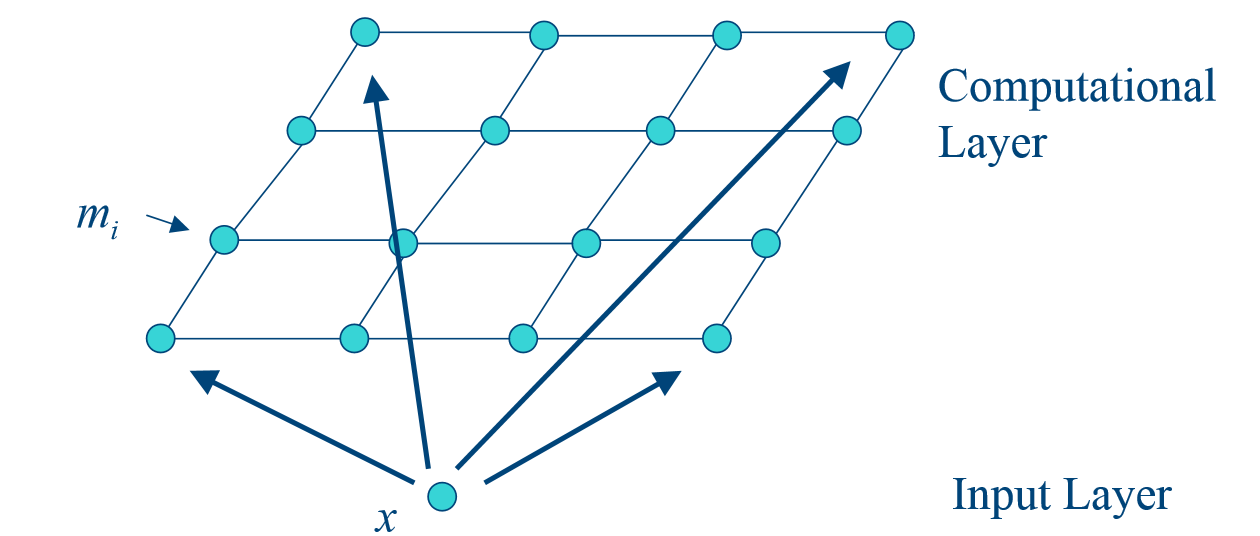
\includegraphics[width=6in,height=3in,keepaspectratio=true]{SOM1.png}
	\caption{Kiến trúc SOM}
  \end{figure}
  \subsubsection{Các thành phần}
  \begin{enumerate}
    \item Tập huấn luyện: 
    Đầu vào bao gồm một tập dữ liệu huấn luyện nhiều phần tử. Mỗi phần tử là một
    Vector có n chiều, và bao gồm p phần tử:
    \[ 
    \begin{bmatrix}
    x_{11} & x_{12} & \dots & x_{1n}\\
    x_{21} & x_{22} & \dots & x_{2n}\\
    \vdots & \vdots & \ddots & \vdots\\
    x_{p1} & x_{p2} & \dots & x_{pn}\\
    \end{bmatrix}
     \]
     \item Bản đồ các neuron: 
     Bản đồ một hoặc hai chiều với thành phần là các neuron với trọng số là một
     Vector có số chiều bằng với phần tử đầu vào
     \[ 
     \begin{bmatrix}
    w_{11} & w_{12} & \dots & w_{1n}\\
    w_{21} & w_{22} & \dots & w_{2n}\\
    \vdots & \vdots & \ddots & \vdots\\
    w_{q1} & w_{q2} & \dots & w_{qn}\\
    \end{bmatrix}
      \]
      Các neuron sẽ hình thành các cụm của bản đồ với mỗi cụm đại diện cho sự tương đồng thuộc tính của các phần tử trong tập huấn luyện. Mỗi cụm bao gồm một hoặc nhiều neuron đại diện. Số neuron được tạo ra ban đầu có thể nhỏ hơn, bằng hoặc lớn hơn số chiều của phần tử đầu vào nhưng phải nhỏ hơn tổng số phần tử của tập huấn luyện.
     \end{enumerate}
   \subsubsection{Các quá trình hình thành thuật toán}
   	 Quá trình tự tổ chức liên quan đến bốn quá trình chính:
   	 \begin{enumerate}
   	 \item Khởi tạo
   	 \begin{itemize}
   	   \item Chọn số lượng neuron thích hợp và số chiều của bản đồ   
   	   \item Tất cả các trọng số kết nối được khởi tạo với giá trị ngẫu nhiên
   	   nhỏ.
   	 \end{itemize}
   	 \begin{figure}[h!]
  	    \centering
	    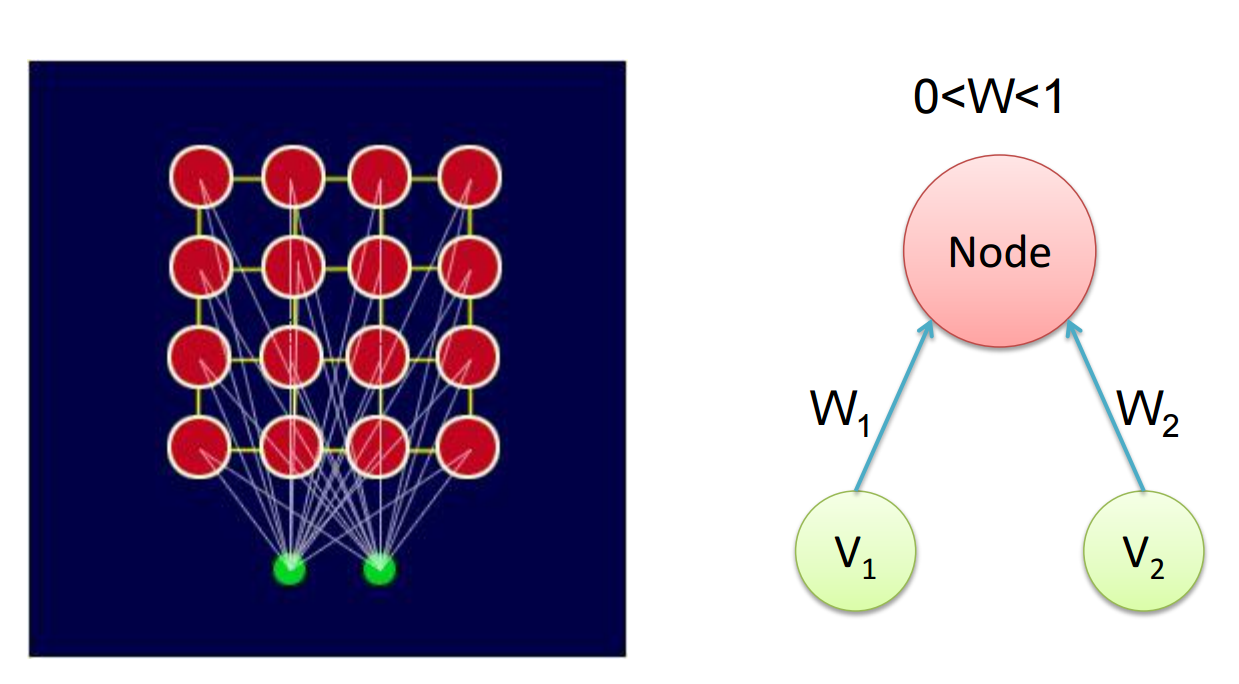
\includegraphics[width=5.5in,height=3.5in,keepaspectratio=true]{SOM2.png}
	    \caption{Khởi tạo SOM}
     \end{figure}
     \item Cạnh tranh\\
     Đối với mỗi mẫu đầu vào, các neuron tính toán giá trị tương ứng của một hàm biệt thức (discriminant function) cung cấp cơ sở cho sự cạnh tranh. Các neuron đặc biệt với giá trị nhỏ nhất của hàm biệt thức được tuyên bố là neuron chiến thắng (winning neuron).
     \item Hợp tác\\
     Các neuron giành chiến thắng xác định các vị trí không gian topo của neuron bị kích thích, do đó cung cấp cơ sở cho việc hợp tác giữa các neuron lân cận.
     \item Thích ứng\\
   	   Các neuron bị kích thích giảm giá trị trọng số về hàm biệt thức liên quan đến mô hình đầu vào thông qua điều chỉnh phù hợp của trọng số kết nối liên quan, như vậy là phản ứng của winning neuron trên các ứng dụng tiếp theo của một mô hình đầu vào tương tự được tăng cường.
   	 \end{enumerate}
	\subsubsection{Thuật toán SOM}
	Thuật toán SOM có thể được chia thành 7 bước:\\
	\textbf{Bước 1} : Số lượng neuron và trọng số của mỗi neuron được khởi tạo.
	Tương đương với quá trình khởi tạo.\\
	\textbf{Bước 2} : Một dữ liệu được chọn ngẫu nhiên từ tập dữ liệu huấn
	luyện và đưa vào mạng.\\
	\textbf{Bước 3} : Mỗi neuron trong mạng được kiểm tra để tính toán mà trọng số
	của nó gần giống như vector đầu vào. Các neuron chiến thắng thường được gọi là
	các đơn vị tốt nhất - Best Matching Unit (BMU). Đây là quá trình cạnh tranh.\\
	\textbf{Bước 4}: Bán kính ảnh hưởng của BMU được tính toán. Giá trị này ban đầu
là khá lớn. Thông thường nó được thiết lập để được bán kính của mạng, giảm dần
từng bước lặp của thuật toán.\\
	\textbf{Bước 5} : Bất kỳ các neuron lân cận được tìm thấy trong vòng bán kính ảnh hưởng của BMU đã tính trong bước 4 được điều chỉnh để làm cho chúng giống như các vector đầu vào. Càng nhiều neuron gần BMU, càng có nhiều trọng số được thay đổi (quá trình cộng tác).\\
	\textbf{Bước 6}: Lặp lại bước 2 với N vòng lặp.\\
	\textbf{Bước 7}: Sau khi kết thúc N vòng lặp, bản đồ đã được định hình thành
	với số cụm nhất định. Mỗi cụm đại diện bởi một hoặc nhiều neuron. Sau đó ta sẽ đưa các phần
tử của tập huấn luyện vào. Nếu neuron nào gần với phần tử đầu vào nhất thì phần
tử đầu vào sẽ thuộc cụm của neuron đó. Sau khi đưa tất cả các phần tử của tập
huấn luyện vào, các phần tử sẽ thuộc vào các cụm. Như vậy ta đã tiến hành phân
cụm thành công các phần tử của tập huấn luyện.     
	\subsubsection{Các quá trình thực hiện} 
	\begin{enumerate}
	  \item Quá trình cạnh tranh - The Competitive Process
	  \begin{itemize}
	    \item Nếu không gian đầu vào là D chiều (tức là D đơn vị đầu vào), có thể viết các
	  mẫu đầu vào như $x=\{x_i\::\:i=1,\dots,D\} $ và trọng số wj của neuron trong
	  lớp tính toán có thể được viết $w_j=\{w_i\::j=1,\dots,N;\:i=1,\dots,D\} $
	  trong đó N là tổng số neuron.
	  \item Sau đó chúng tôi có thể xác định chức năng biệt thức của
	  chúng tôi là khoảng cách Euclide bình phương giữa các vector đầu vào x và wj vector trọng số cho mỗi neuron j
	  \[ d_j(x) = \sum_{i=1}^D (x_i - w_{ji})^2 \]
	  \item Phương trình được tính bằng công thức khoảng cách Euclide bình phương
	  vì ta không quan tâm đến khoảng cách thực tế từ đầu vào. Chúng ta chỉ cần một số loại quy mô thống nhất để so sánh mỗi nút với vector đầu vào. Nói cách khác, các neuron có trọng số vector gần nhất với vector đầu vào được xác định là winning neuron.
	  \item Bằng cách này, không gian đầu vào liên tục có thể được ánh xạ vào không gian đầu ra rời rạc của neuron của một quá trình đơn giản của cuộc cạnh tranh giữa các neuron.
	  \end{itemize}
	  \item Quá trình hợp tác - The Cooperative Process\\
	  Trong các nghiên cứu sinh học thần kinh chúng ta thấy rằng có sự tương tác
	  bên trong một tập hợp các neuron bị kích thích. Khi một neuron hoạt động, các
	  neuron lân cận của nó có xu hướng dễ kích thích hơn so với những neuron ở
	  xa.
	  Có một topo lân cận phân rã theo khoảng cách. Chúng ta áp dụng lý thuyết đó
	  vào SOM với công thức
	  \[ T_{j,I(x)}=e^{-\frac{S_{j,I(x)}^2}{2\sigma^2}} \]
	  \begin{itemize}
	    \item $T_{j,I(x)}$ sử dụng để xác định các neuron gần với winning neuron
	    nhiều hơn các neuron khác nằm ngoài bán kính ảnh hưởng. Các neuron bên
	    ngoài bán kính ảnh hưởng được bỏ qua hoàn toàn.
	    \item $I(x)$ là vị trí của winning neuron. Điều này có một số đặc tính quan
	    trọng: nó là tối đa tại các neuron chiến thắng, nó là đối xứng về neuron đó, nó
	    làm giảm về giá trị 0 khi khoảng cách đi đến vô cùng, và nó không di chuyển 
	    (nghĩa là độc lập với vị trí của các neuron chiến thắng).
	    \item Trong đó $\sigma$ là bán kính ảnh hưởng của neuron
	    \[ \sigma(t) = \sigma_0 e^{\frac{-t}{\lambda}} \]
	    \tab t: vòng lặp hiện tại\\
	    \tab $\lambda$: hằng số = số vòng lặp / kích thước bản đồ $\sigma_0$. Giá
	    trị gần như là tùy ý. Bất kỳ giá trị hằng số nào cũng có thể được lựa chọn.
	    Tuy nhiên nó phụ thuộc trực tiếp vào kích thước bản đồ và số lần lặp để
	    thực hiện.\\
	    \tab $\sigma_0$: bán kính ảnh hưởng của neuron tại thờ điểm $t_0$ 
	  \end{itemize}
	  Một thuộc tính đặc biệt của SOM là $\sigma$ kích thước của bán kính ảnh hưởng
	  cần phải giảm theo thời gian. Một hàm thời gian phụ thuộc phổ biến là một
	  phân rã theo hàm số mũ.\\\\
	  Tại t = 0 giá trị là lớn nhất. Khi t (số lần lặp hiện hành) tăng lên,
	  giá trị tiệm cận bằng không. Đây chính là điều chúng ta muốn. Bán kính bắt
	  đầu như bán kính của mạng tinh thể, khi tiệm cận bằng không, lúc đó bán kính chỉ đơn giản là nút BMU\\
	  $S_{j,I(x)}$ là khoảng cách Euclid từ neuron lân cận đến winning neuron
	  \item Quá trình thích ứng - The Adaptive Process\\
	  Không phải chỉ có winning neuron được cập nhật trọng số mà các neuron lân cận
	  cũng được cập nhật. Trong thực tế, phương trình cập nhật trọng số thích hợp
	  là 
	  \[ \Delta w_{ji} = \eta(t).T_{j,I(x)} . (x_i - w_{ji})  \]
	  \[ w_{ji} = w_{ji} + \Delta w_{ji} \]
	  $\eta(t)$: tốc độ học tập - learning rate. Với $\eta(t+1) = \alpha
	  \eta(t)^{k/k_{max}}$ trong đó $0 \leq \alpha \leq 1$ quyết định lượng giảm
	  tốc độ học, k là số lần lặp của thuật toán đã được chạy, và $k_{max}$ là
	  thông số khi muốn việc học dừng lại.\\\\ 
	  Mỗi lần cập nhật trọng số học tập là để di chuyển các vector trọng số $w_i$
	  của winning neuron và các neuron lân cận về phía vector đầu vào x. Quá trình lặp
	  đi lặp lại của dữ liệu huấn luyện do đó dẫn đến trật tự topo.\\\\ 
	  Có hai giai đoạn mang tính chất của quá trình thích nghi này:
	  \begin{itemize}
	    \item Thứ tự hoặc giai đoạn tự tổ chức (Ordering or self-organizing phase )
	    - trong đó thứ tự topo của vector trọng số diễn ra. Thông thường điều này
	    sẽ mất là 1000 lần lặp lại các thuật toán SOM, và xem xét cẩn thận cần phải
	    được đưa ra để lựa chọn bán kính ảnh hưởng và tham số tốc độ học.
	    \item Hội tụ - trong đó các bản đồ feature được tinh chỉnh và đến khi cung
	    cấp một lượng thống kê chính xác về không gian đầu vào. Thông thường các số lần lặp lại trong giai đoạn này sẽ có ít nhất hơn 500 lần số lượng neuron trong mạng, và một lần nữa các thông số phải được lựa chọn cẩn thận.
	  \end{itemize}
	\end{enumerate}
\subsection{Ví dụ của SOM}
\begin{figure}[h!]
  \begin{minipage}{0.4\textwidth}
	\centering
    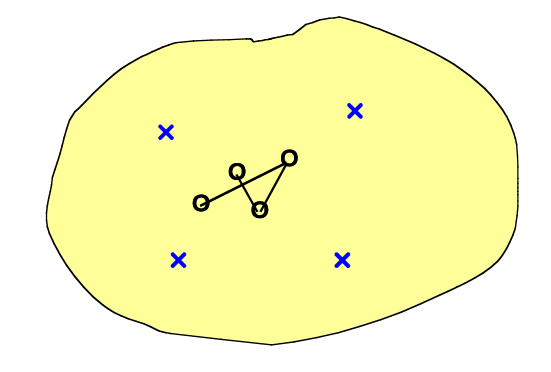
\includegraphics[width=1\textwidth,keepaspectratio=true]{SOM6.png}
    \caption{Bước 1: Khởi tạo giá trị bảng đầu}
  \end{minipage}
  ~
  \begin{minipage}{0.1\textwidth}
  \end{minipage}
  ~
  \begin{minipage}{0.5\textwidth}
  Giả sử ta có bốn điểm dữ liệu trong không gian đầu vào hai chiều liên tục, và muốn đưa vào bốn điểm trong một không gian đầu ra một chiều rời rạc. Các nút đầu ra (neuron) được đưa các điểm trong không gian đầu vào (vòng tròn). Trọng số ban đầu được chọn ngẫu nhiên là vòng tròn tại các vị trí ngẫu nhiên trong trung tâm của không gian đầu vào. 
  \end{minipage}
\end{figure}
\begin{figure}[h!]
  \begin{minipage}{0.4\textwidth}
	\centering
    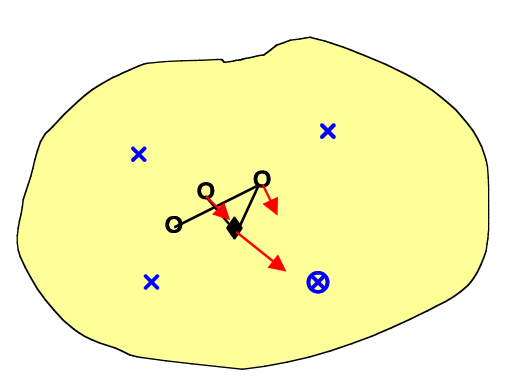
\includegraphics[width=1\textwidth,keepaspectratio=true]{SOM3.png}
    \caption{Bước 2: Đưa giá trị đầu vào học}
  \end{minipage}
  ~
  \begin{minipage}{0.1\textwidth}
  \end{minipage}
  ~
  \begin{minipage}{0.5\textwidth}
  Ta chọn ngẫu nhiên một trong những điểm dữ liệu cho vào học (kí hiệu là vòng tròn bao quanh dấu x). Các điểm đầu ra gần nhất đại diện cho các neuron chiến thắng (tứ giác được tô đen). Đó là winning neuron đang di chuyển về phía điểm dữ liệu bằng lượng nhất định, và hai neuron lân cận di chuyển bởi một lượng nhỏ hơn (mũi tên).
  \end{minipage}
\end{figure}
\begin{figure}[h!]
  \begin{minipage}{0.4\textwidth}
	\centering
    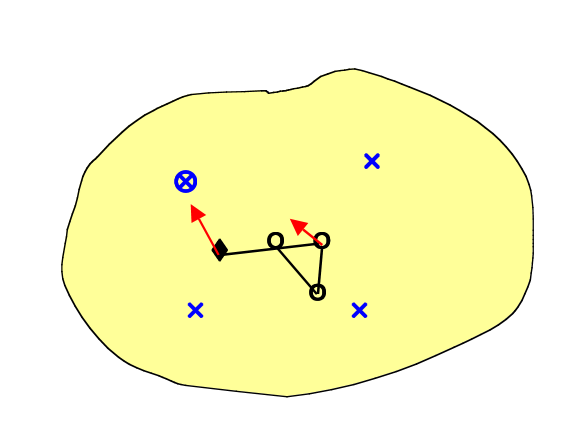
\includegraphics[width=1\textwidth,keepaspectratio=true]{SOM4.png}
    \caption{Bước 3: Học giá trị tiếp theo}
  \end{minipage}
  ~
  \begin{minipage}{0.1\textwidth}
  \end{minipage}
  ~
  \begin{minipage}{0.5\textwidth}
  Tiếp tục chọn ngẫu nhiên một điểm dữ liệu cho vào học (qua trong vòng tròn).
  Winning neuron đang tiến về điểm đầu vào bằng lượng nhất định, và neuron lân cận di chuyển bởi một lượng nhỏ hơn (mũi tên).
  \end{minipage}
\end{figure}
 \vfill
\begin{figure}[h!]
  \begin{minipage}{0.4\textwidth}
	\centering
    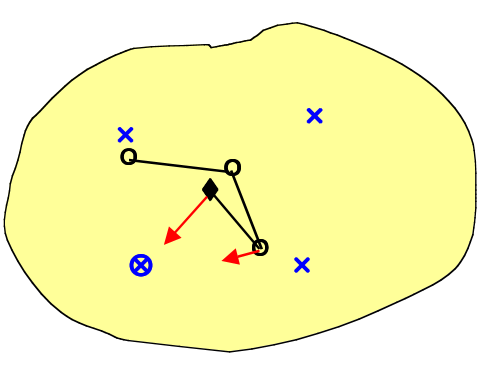
\includegraphics[width=1\textwidth,keepaspectratio=true]{SOM5.png}
    \caption{Bước 4: Tiếp tục cho các giá trị vào học}
  \end{minipage}
  ~
  \begin{minipage}{0.6\textwidth}
  Tiếp tục chọn ngẫu nhiên một điểm dữ liệu cho học (qua trong vòng tròn).
  Winning neuron đang tiến về điểm dữ liệu bằng một lượng nhất định, và một
  trong những neuron láng giềng di chuyển bởi một số lượng nhỏ hơn (mũi
  tên).
  Cuối cùng toàn bộ lưới được xác định để đại diện cho không gian đầu vào.
  \end{minipage}
\end{figure}

\subsection{Ứng dụng của SOM}
  SOM thường được sử dụng làm công cụ trực quan. Nó giúp chúng ta hình dung dễ
  dàng về mối quan hệ giữa khối lượng lớn dữ liệu.\\ 
\begin{figure}[h!]
	\centering
    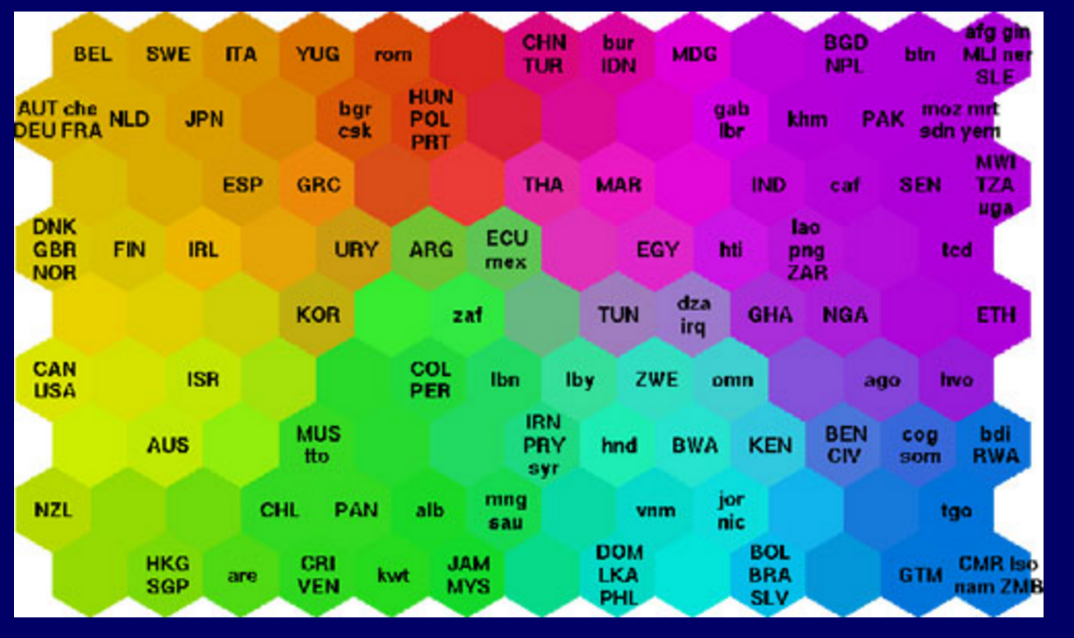
\includegraphics[width=5in,keepaspectratio=true]{SOM_ex1.png}
    \caption{Biểu đồ thể hiện chất lượng cuộc sống các quốc gia}
\end{figure}
SOM đã được sử dụng để phân loại dữ liệu thống kê mô tả khác nhau chất lượng của
cuộc sống theo các yếu tố như tình trạng sức khỏe, dinh dưỡng, các dịch vụ giáo
dục, \ldots. Các quốc gia có chất lượng cuộc sống với các yếu tố tương tự cùng
nhóm nhau. Các quốc gia có chất lượng cuộc sống tốt hơn nằm phía trên bên trái và các nước nghèo khó nhất nằm ở phía dưới bên phải. Lưới lục giác là một ma trận khoảng cách thống nhất, thường được biết đến như một U-ma trận. Mỗi hình lục giác đại diện cho một nút trong SOM\\
Ngoài ra còn có một số ứng dụng khác như phân loại hình ảnh hay màu sắc.
\begin{figure}[h!]
	\centering
    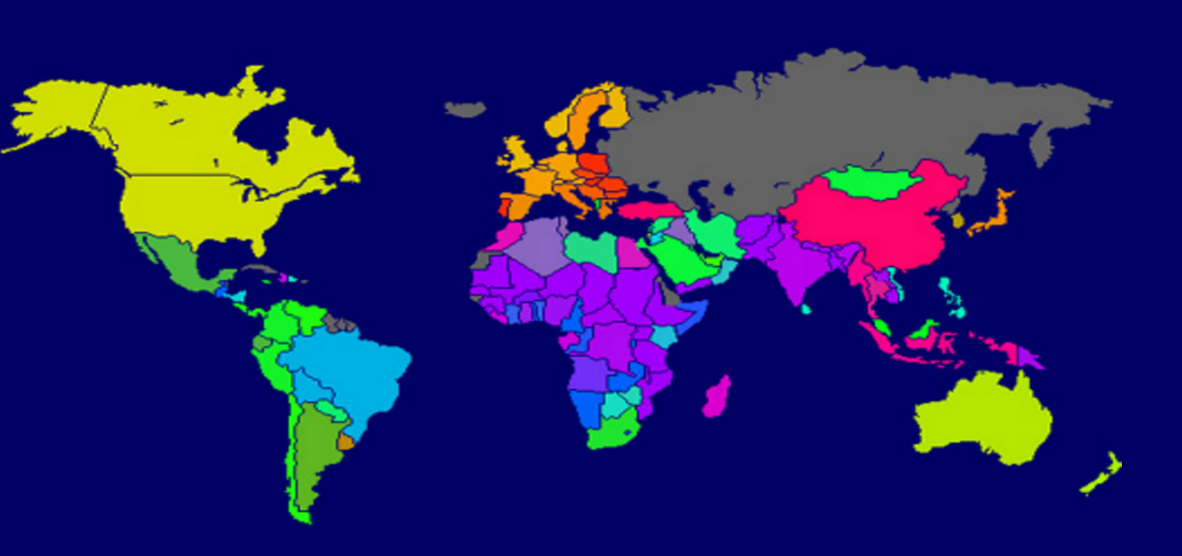
\includegraphics[width=5in,keepaspectratio=true]{SOM_ex2.png}
    \caption{Bản đồ chất lượng cuộc sống thế giới}
\end{figure}
\chapter{Hệ thống phát hiện xâm nhập OSSEC}
\section{Tổng quan về OSSEC}
  OSSEC HIDS (Open Source HIDS) là 1 HIDS mã nguồn mở, đa nền tảng và có tính mở rộng cao.
OSSEC cung cấp các chức năng để giám sát hoạt động trên máy tính và từ đó đảm
bảo an toàn cũng như bảo mật cho máy tính.\\\\
  OSSEC có các chức năng chính như sau:
  \begin{itemize}
    \item Công cụ phân tích mạnh mẽ
    \item Tích hợp phân tích file log
    \item Kiểm tra tính toàn vẹn của file
    \item Giám sát thanh ghi trên Windows
    \item Cung cấp cơ chế quy định tập trung (policy centralize)
    \item Kiểm tra rootkit
    \item Phát cảnh báo thời gian thực
    \item Active response
  \end{itemize}
  OSSEC có thể chạy trên nhiều hệ điều hành khác nhau, bao gồm Linux, OpenBSD,
  FreeBSD, Mac OS X, Sun Solaris, và cả Microsoft Windows.\\\\
OSSEC được xây dựng dựa trên ngôn ngữ C, các file cấu hình và file rules được
lưu trữ dưới dạng xml, cấu trúc tổ chức này giúp việc cấu hình dễ hiểu, dễ chỉnh
sửa.
\section{Mô hình của OSSEC}
  \subsection{Mô hình local}
    \begin{itemize}
      \item Mô hình local thích hợp khi cài đặt lên hệ thống chỉ có 1 máy tính, ví dụ
    như máy tính cá nhân, hoặc là server riêng lẻ.
    \item Mô hình local dễ dàng quản lý và có thể chỉnh sửa theo ý muốn ngay trên thiết
bị cài đặt.
	\item Với mô hình local, máy tính được cài đặt OSSEC sẽ có đầy đủ các tính năng
cung cấp bởi OSSEC.
    \end{itemize}
    
	\subsection{Mô hình server}
	\begin{figure}[h!]
	\centering 
	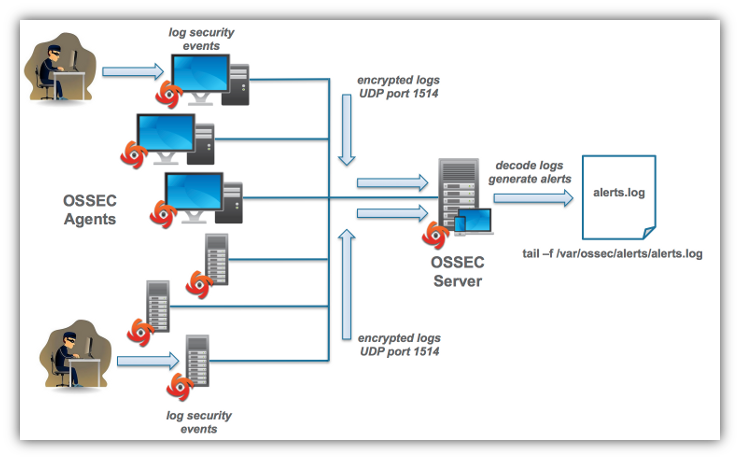
\includegraphics[width=6in,height=3in,keepaspectratio=true]{server-agent.png}
	\caption{Mô hình Server-agent trong OSSEC}
\end{figure}
	\begin{itemize}
	  \item Mô hình server-agent thích hợp khi cài đặt lên hệ thống có nhiều máy tính, ví
	như như trong 1 công ty, 1 phòng nghiên cứu, nhằm mục đích quản lý tập trung
	toàn bộ hệ thống. Mô hình này đòi hỏi thiết lập 1 máy tính đóng vai trò server, và các máy tính còn lại là các agent.
	\item Về phía server: Server sẽ có đầy đủ tính năng của OSSEC, như việc kiểm tra
	 toàn vẹn file, giám sát thanh ghi, phát hiện rootkit,... ngoài ra có thêm các
	 chức năng như thu thập log file, ghi file log cảnh báo, đặt luật cho toàn bộ hệ thống IDS.
	 \item Về phía agent:
Agent chỉ có các chức năng sau:
kiểm tra toàn vẹn file,
giám sát thanh ghi,
phát hiện rootkit,
active response.
Các chức năng như ghi file log cảnh báo, xem file log, thu thập syslog, đặt luật
đều được tập trung tại server.
\item Mô hình này cung cấp khả năng triển khai hệ thống an ninh để bảo vệ hệ thống
trên các máy tính và tập trung dữ liệu xử lý trên server, các agent sẽ loại bỏ
được công việc xử lý dữ liệu, và cơ chế tập trung về quy định và xử lý giúp quản
lý tốt hơn.   
	\end{itemize}
  
\section{Cách thức hoạt động trong OSSEC}
  \begin{figure}[h!]
	\centering 
	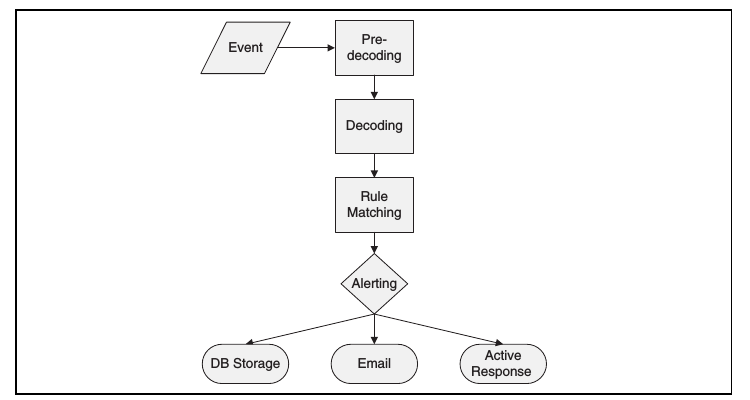
\includegraphics[width=6in,height=3in,keepaspectratio=true]{eventFlow.png}
	\caption{Cách thức hoạt động của OSSEC}
  \end{figure}
  
     \subsection{Nhận event}
     Event là những log file của các chương trình khi được thực thi, các
     chương trình trên máy tính khi thực thi đều tạo ra file log để ghi lại hành
     động.\\
     Chương trình OSSEC sẽ đọc tất cả các log file này mỗi khi chương
     trình khác thực thi. Từ file log này, OSSEC sẽ thực hiện công việc tiếp theo.
     \subsection{Rút trích dữ liệu}
     Tiến hành Decode và rút trích những thông tin liên quan từ event,
     phần decode được thực hiện thông qua 2 giai đoạn:\\
       \subsubsection{Predecoding}
       Rút trích các thông tin static từ event từ các trường
       quen thuộc và đơn giản, như ngày, giờ, log, hostname, tên chương trình.
       \begin{figure}[h!]
	\centering 
\fbox{	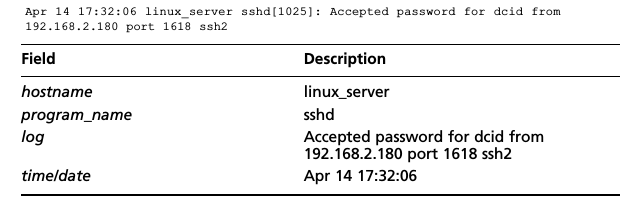
\includegraphics[width=6in,height=3in,keepaspectratio=true]{predecode_example.png}}
	\caption{Predecoder}
  \end{figure}\\
Predecoding hoạt động không dựa vào nguồn dữ liệu đầu vào của
         event. Vì tất cả các event đều sẽ có chung các thông tin đơn giản mà
         predecoding rút trích.\\\\
        Khi xử lý log: OSSEC sẽ chuẩn hóa các kiểu log khác nhau thành 1
         kiểu chuẩn do OSSEC định nghĩa, từ đó có thể viết các rules theo kiểu
         chuẩn này để rút trích được các thông tin cần thiết. Ngoài ra còn có
         thể định nghĩa rule để xét từng trường riêng với nhau: hostname hoặc
         program\_name.\\\\ 
         Ví dụ: Syslog ở hình trên và ASL ở hình dưới có log file hoàn toàn khác
         nhau, nhưng cũng có thể rút trích được theo các trường như decoder ở
         trên.
          \begin{figure}[h!]
	\centering 
\fbox{	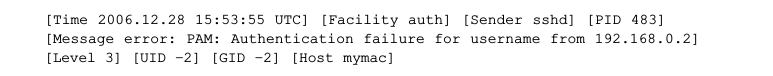
\includegraphics[width=6in,height=3in,keepaspectratio=true]{predoced_another_ASL.png}}
	\caption{Log của ASL}
  \end{figure}
  		\subsubsection{Decoding}
  		Đây là bộ phận quan trọng nhất trong quá trình hoạt động của OSSEC, các
  		thông tin quan trọng để xác định sự kiện được lấy ra trong quá trình
  		này.\\\\
  		Decoding rút
  		trích những thông tin mà phần predecoding chưa lấy được, như usernames hoặc địa chỉ IP nguồn, \ldots \\\\
  		Khác với predecoder, các thông tin do decoder rút trích khác nhau giữa các
  		event, do vậy mỗi 1 event đều có 1 decoder riêng, toàn bộ các decoder đều
  		được đặc tả trong file decoders.xml.\\\\
  	 Các trường có trong 1 decoder được miêu tả trong bảng dưới.
  	 \begin{table}[h]
  	 	\centering
		\begin{tabular}{|p{3cm}|p{10cm}|}
		
  			\hline
  			\textbf{Tag} & \textbf{Miêu tả}\\
		 \hline
  			program\_name & Thực thi decoder khi tên chương trình trong file log
  			trùng với program\_name\\
  			\hline
  			prematch & Thực thi decoder khi prematch trùng với bất kỳ phần nào trong
  			log\\
  			\hline
  			regex & Regular Expression để so sánh với log, rút trích những dữ liệu   			trùng
  			\\
  			\hline 
  			offset & Thuộc tính của regex. Để báo so sánh regex bắt đầu từ đâu, có 2
  			giá trị là after\_prematch và after\_parent\\
  			\hline
  			order & Thứ tự trong regex khi rút trích dữ liệu. Có thể là sự kiện
  			thường gặp (srcip, user, dstip, dstport, \dots)\\
  			\hline
  			parent & Decoder cha trước khi xét đến decoder này.\\
  			\hline  
  		\end{tabular}
  		\caption{Các trường trong decoder}
	\end{table}\\
	Với những trường này, decoder cung cấp các tính năng như so sánh theo tên
	chương trình (program\_name) hoặc so trùng thông tin (prematch). Ngoài ra
	decoder còn xếp sắp theo nhiều cấp trong mô hình cây giúp cho việc tạo decoder
	dễ dàng hơn, có tính kế thừa và mở rộng cao.\\\\
	 Dưới đây là 1 ví dụ về decoder của 1 đoạn log của ACL. Trong đoạn log sử dụng
  các tag \textless parent\textgreater{} để kế thừa decoder cha, \textless
  type\textgreater{} để xét định loại decoder, xác định tường để so sánh bằng
  \textless prematch\textgreater, sau đó xác định thông tin cần rút trích bằng \textless regex\textgreater{} và
  \textless order\textgreater.
	\begin{figure}[h!]
	\centering 
\fbox{	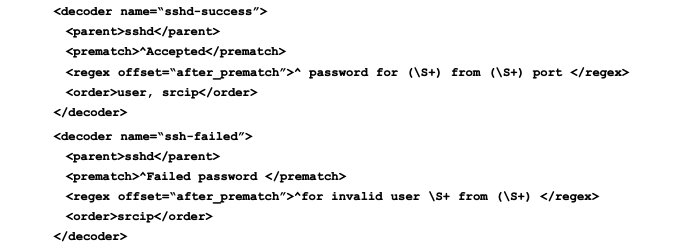
\includegraphics[width=6in,height=3in,keepaspectratio=true]{decoder_parent.png}}
	\caption{Decoder}
  \end{figure}
 
   \begin{figure}[h!]
	\centering 
\fbox{	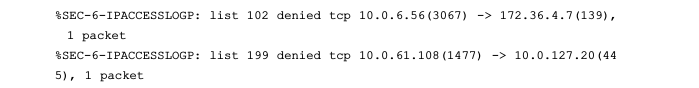
\includegraphics[width=6in,height=3in,keepaspectratio=true]{logACL.png}}
	\caption{Đoạn log của ACL}
	\end{figure}
	\begin{figure}[h!]
	\centering 
\fbox{	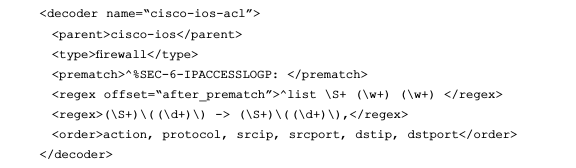
\includegraphics[width=6in,height=3in,keepaspectratio=true]{decoACL.png}}
	\caption{Decoder cho đoạn log ACL}
  \end{figure}
       \subsection{Rule matching}
        Sau khi rút trích được dữ liệu từ event, 1 cơ
       chế so sánh rules được gọi để xác định tính chất của event và quyết định điều khiển báo động.
\section{Về rules trong OSSEC}
Rules được định nghĩa trong các file xml riêng cho từng vấn đề (apache,
syslog, \dots), 1 file chứa nhiều rule.\\\\  
Mỗi rules được gán 1 ID cố
định và 1 mức độ (level) của rules đó.
  \subsection{ Về ID}
  \begin{itemize}
    \item Rules trong OSSEC có ID từ 00000 đến 50799, các rule được chia nhóm
    theo từng chức năng riêng, có các nhóm quan trọng như:
    \begin{itemize}
      \item 01000 - 01999: Rule cho syslog
      \item 05100 - 05299: Rule cho nhân hệ thống Linux, UNIX, BSD
      \item 30100 - 30999: Rule cho Apache HTTP server
      \item 31100 - 31199: Rule cho truy cập web 
      \item 50100 - 50299: Rule cho MySQL database
      \end{itemize}
      \item Ngoài ra, người dùng có thể tự định nghĩa rule có ID từ 100000 đến
      119999
      \item Khi sử dụng mô hình server-agent, các agent có thể có rules riêng
      cho bản thân, các rules này sẽ được viết vào trong file local\_rules.xml.
  \end{itemize}
  \subsection{Về mức}
  \begin{itemize}
    \item OSSEC gồm có 16 mức: 0 - 15, số mức cáng cao càng có độ cảnh báo cao.
    \item Mức 0 là mức đặc biệt, mang ý nghĩa là bỏ qua. Khi 1 rules được đánh
    giá là mức 0, event đó sẽ được bỏ qua và không xét tới nữa.
    \item Các luật trong OSSEC được lưu trữ theo cấu trúc cây, luật với mức cao
    được đánh giá trước, nhưng trước tiên phải xét luật với mức 0 vì đây là trường hợp đặc biệt, sẽ bỏ qua tất cả.
  \end{itemize}
  \subsection{Atomic rules}
  \begin{itemize}
    \item Là các luật chỉ xét riêng cho từng event riêng lẻ.
    \item Các tag chính trong rule:
    \begin{itemize}
      \item Tất cả các rule trong OSSEC đều được đặt trong tag \textless
      group\textgreater, \textless group\textgreater{} là tag để quản lý các
      loại rule có chung đặc điểm, mỗi group có tên để nêu lên đặc điểm của rule trong đó, như syslog, sshd, \dots
      \item Trong OSSEC cung cấp cơ chế kế thừa giữa các rules, 1 event sau khi
      được rút trích, thông tin đó sẽ được so sánh với rule cha, nếu trùng sẽ so
      sánh tiếp xuống rule con, như vậy sẽ tiết kiếm được chi phí so sánh khi
      không cần thiết phải so sánh hết với toàn bộ tập rule, và sẽ cung cấp khả
      năng để các rules mở rộng theo nhiều hướng từ 1 rules chính. Sử dụng thừa
      kế bằng cách thừa kế group chứa rule với tag \textless group\textgreater.
      \item Có các group lớn mà OSSEC đã định nghĩa sẵn, có thể sử dụng những
      group này làm group cha khi người dùng tự định nghĩa các rule.
      \begin{figure}[h!]
	\centering 
\fbox{	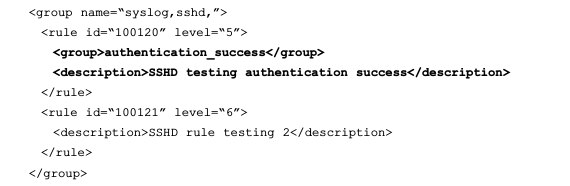
\includegraphics[width=6in,height=3in,keepaspectratio=true]{rule_subgroup.png}}
	\caption{Subgroup trong group}
  \end{figure}
      \item Sử dụng tag \textless decoded\_as\textgreater{}  để xác định decoder
      để decode event, rule được xác định decoder chỉ so sánh khi được decoder đó decode.
      \item Sử dụng tag \textless match\textgreater{}  để hỗ trợ cho tag \textless
      decoder\_as\textgreater, tag \textless match\textgreater{}  để so sánh trùng với nội dung mà decoder rút trích được. 
      \begin{figure}[h!]
	\centering 
\fbox{	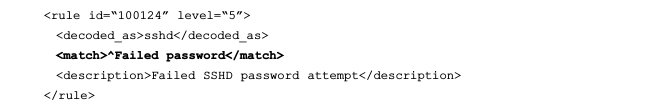
\includegraphics[width=6in,height=3in,keepaspectratio=true]{rule_match.png}}
	\caption{Tag match trong rule}
  \end{figure}
  	  \item Ngoài ra còn có các tag như \textless hostname\textgreater,
  	  \textless srcip\textgreater{}   để kiểm tra cụ thể theo yêu cầu như hostname hoặc srouce ip.
  	  \begin{figure}[h!]
	\centering 
\fbox{	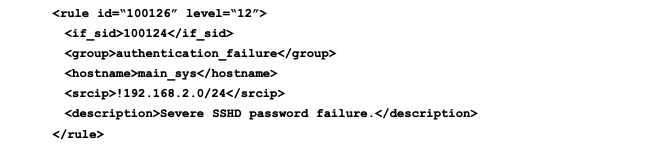
\includegraphics[width=6in,height=3in,keepaspectratio=true]{rule_scrip.png}}
	\caption{Tag scrip trong rule}
  \end{figure}
      \item Tag \textless time\textgreater{}  để kiểm tra về thời gian của event, để xác định chính
      xác hơn về quy định. Ví dụ như việc login vào server chỉ nên xảy ra trong thời gian làm việc, việc mọi sự đăng nhập ngoài giờ làm việc sẽ được cảnh báo ở mức cao hơn.
      \begin{figure}[h!]
	\centering 
\fbox{	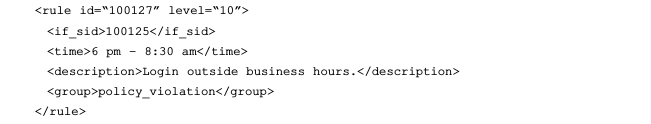
\includegraphics[width=6in,height=3in,keepaspectratio=true]{rule_time.png}}
	\caption{Tag time trong rule}
  \end{figure}
      \item Lưu ý là 1 sự kiện chỉ tạo ra 1 alert, rule được so sánh theo sơ đồ
      cây và node cuối cùng được so sánh trùng sẽ phát ra alert với mức của rule đó.
    \end{itemize}
  \end{itemize}
  \subsection{Composite rules}
  \begin{itemize}
    \item  Composite rules không xét có event riêng lẻ với nhau, mà so sánh
    event hiện tại với các event đã bắt được trước đó. Để các rule có để giữ được trạng thái, 1 rule phải có thêm hai thuộc tính sau:
    \begin{itemize}
      \item Frequency: để lấy tần số xuất hiện của event (event/pattern), tần số
      đủ lớn mới cảnh báo.
      \item Timeframe: xem xét lại thời gian từ event bây giờ tới thời điểm
      event trước đó  là bao nhiêu giây.
      \end{itemize}
      \begin{figure}[h!]
	\centering 
\fbox{	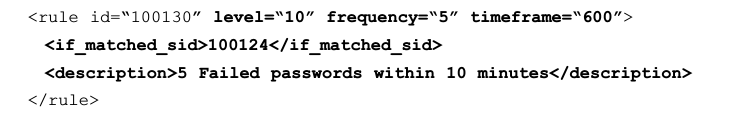
\includegraphics[width=6in,height=3in,keepaspectratio=true]{fre_time.png}}
	\caption{Tần số trong composite rule}
  \end{figure}
    \item Event được đếm tần số xuất hiện có thể dựa trên id \textless
    if\_match\_sid\textgreater, dựa trên group \textless
    if\_match\_group\textgreater, dựa trên regex \textless
    if\_match\_regex\textgreater.
    \item Ngoài ra có thể tăng độ chính xác và giảm lỗi bằng các tag so sánh
    cùng ip, port, hostname, program name.
     \begin{table}[h]
  	 	\centering
		\begin{tabular}{|p{3cm}|p{10cm}|}
		\hline
		\textbf{Tag} & \textbf{Miêu tả}\\
		 \hline
		 same\_source\_ip & Địa chỉ IP của Source phải giống nhau\\
		 \hline
		 same\_dest\_ip & Địa chỉ IP của Dest phải giống nhau\\
		 \hline
		 same\_src\_port & Địa chỉ Port của Source phải giống nhau\\
		 \hline
		 same\_dst\_port & Địa chỉ Port của Dest phải giống nhau\\
		 \hline
		 same\_location & Phải cùng 1 host hoặc agent\\
		 \hline
		 same\_user & Username được rút trích phải giống nhau\\
		 \hline
		 same\_id & ID được rút trích phải giống nhau\\
		 \hline
		\end{tabular}
		\caption{Các tag trong composite rule}
	  \end{table}
  \end{itemize}\vfill
\section{Cách thức cấu hình để OSSEC hoạt động}
Tất cả các cấu hình cơ bản cho OSSEC đều nằm trong file ossec.conf, file này
được viết bằng xml. File cấu trúc xml được chọn vì nhiều lý do: dễ đọc và dễ tìm
kiếm tới những phần cụ thể, cấu trúc kế thừa trong xml giúp cho việc xác định
nơi bắt đầu và kết thúc của từng phần cấu hình dễ dàng hơn, file xml có thể được
ghi 1 cách tự động từ chương trình cũng có thể dễ dàng thay đổi từ bất cứ 1 công
cụ đọc text nào.\\\\ 
Trong file ossec.conf có các tag lớn sau:
\begin{table}[h!]
  	 	\centering
		\begin{tabular}{|p{4cm}|p{9cm}|}
		\hline
		\textbf{Thành phần} & \textbf{Miêu tả}\\
		 \hline
		 \textless global\textgreater & Những cấu hình chung cho hệ thống trong mô
		 hình local hoặc là riêng server\\
		 \hline
		 \textless alerts\textgreater & Tùy chọn cho cảnh báo email và log\\
		 \hline
		 \textless email\_alerts\textgreater & Tùy chọn chi tiết cho cảnh báo email\\
		 \hline
		 \textless remote\textgreater & Cấu hình riêng cho các agent từ xa (chỉ áp
		 dụng cho server)\\
		 \hline
		 \textless database\_output\textgreater & Tùy chọn cho việc ghi log vào trong
		 database\\
		 \hline
		 \textless rules\textgreater & Liệt kê tất cả những file rule được sử dụng\\
		 \hline
		 \textless client\textgreater & Cấu hình liên quan đến agent\\
		 \hline
		 \textless localfile\textgreater & Cấu hình cho việc giám sát log file\\
		 \hline
		 \textless syscheck\textgreater & Cấu hình cho việc kiểm tra tính toàn vẹn\\
		 \hline
		 \textless rootcheck\textgreater & Cấu hình cho việc kiểm tra rootkit và điều
		 lệ\\
		 \hline
		 \textless command\textgreater & Cấu hình cho active response\\
		 \hline
		 \textless active-response\textgreater & Cấu hình nâng cao cho active
		 response\\
		 \hline
		 \end{tabular}
		 \caption{Các thành phần trong file ossec.conf}
\end{table}\\
  Cách thức cấu hình cụ thể sẽ được trình bày theo từng module riêng trong
mục các module trong OSSEC.
\section{Các module trong OSSEC}
  \subsection{Log alert và email alert}
  \begin{itemize}
    \item Đây là module cơ bản và quan trọng nhất trong OSSEC, cần điều chỉnh module này phù hợp với hệ thống cài đặt để tối ưu theo ý muốn người sử dụng.
    \item Theo mặc định, khi event tạo ra alert với mức từ 1 đến 15 đều được OSSEC ghi vào trong log file. Các sự kiện trên mức 7 sẽ được OSSEC gửi email để alert cho admin.
    \item Để thay đổi mức cảnh báo này, có thể sử dụng 2 trường trong tag
    \textless alert\textgreater, đó là \textless log\_alert\_level\textgreater{} và
    \textless email\_alert\_level\textgreater.
    \begin{figure}[h!]
	\centering 
\fbox{	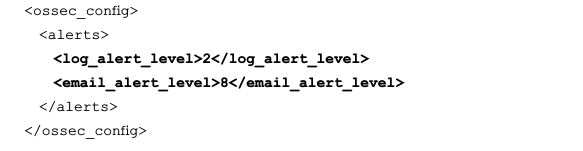
\includegraphics[width=6in,height=3in,keepaspectratio=true]{mail_alert.png}}
	\caption{Cấu hình mức cảnh báo email của OSSEC}
  \end{figure}
     \item Email alert là 1 tính năng rất hữu dụng trong OSSEC, vì nó cung cấp
     khả năng phản ứng nhanh chóng với các cảnh báo.
     \item Để cấu hình tính năng email alert, sử dụng các tag trong tag
     \textless global\textgreater.
     \begin{figure}[h!]
	\centering 
\fbox{	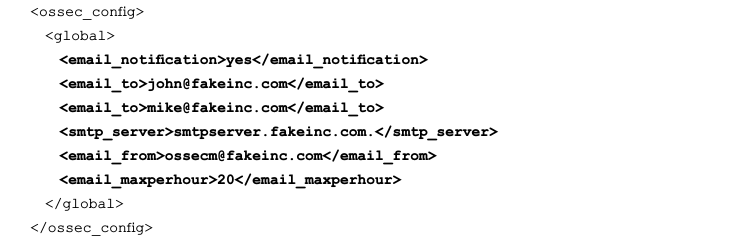
\includegraphics[width=6in,height=3in,keepaspectratio=true]{email_name.png}}
	\caption{Cấu hình email cảnh báo trong OSSEC}
  \end{figure}
  \item Ngoài ra còn có các tính năng hỗ trợ thêm trong tag
  \textless email\_alerts\textgreater:
  \begin{itemize}
    \item Tag \textless group\textgreater: xác định nhóm alert của chương trình
    nào sẽ gửi email đến địa chỉ trên.
    \item Tag \textless level\textgreater: xác định mức của cảnh báo để gửi
    email.
    \item Tag \textless format\textgreater: xác định cách thức gửi cảnh báo. Sms
    để gửi cảnh báo bằng tin nhắn.
    \item Tag \textless event\_location\textgreater: xác định chỉ những cảnh báo
    đến từ các agent nào mới gửi cảnh báo.
    \end{itemize}
  \end{itemize}
  \subsection{Xác định file rules}
  Trong OSSEC cho phép include các file rules cần thiết để xác định rule nào
  được kiểm tra, các file rule đều nằm trong đường dẫn ossec/rules. File rules
  được xác định phải nằm trong tag \textless include\textgreater.
  \begin{figure}[h!]
	\centering 
\fbox{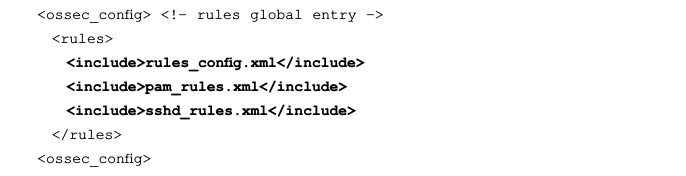
\includegraphics[width=6in,height=3in,keepaspectratio=true]{conf_rule.png}}
	\caption{Liệt kê file rule trong ossec.conf}
  \end{figure}
  \subsection{Kiểm tra toàn vẹn hệ thống}
  \begin{itemize}
    \item Phần cơ bản và quan trọng nhất trong 1 HIDS, cơ bản là kiểm tra
    checksum của file so với checksum bản file tốt để xem file có bị thay đổi hay không.
    \item Kiểm tra toàn vẹn file có thể giúp chống lại các loại trojans, phần
    mềm độc hại có khả năng thay đổi mã chương trình.
    \item Trong OSSEC việc kiểm tra tính toàn vẹn thông qua 3 tag chính trong
    tag \textless syscheck\textgreater:
    \begin{itemize}
      \item Tag \textless directory\textgreater: cung cấp cơ chế để xác định
      folder được kiểm tra toàn vẹn.
      \item Tag \textless ignore\textgreater: xác định file, folder có thể bỏ qua trong
      lúc kiểm tra.
      \item Tag \textless frequency\textgreater: xác định tần số kiểm tra.
    \end{itemize}
    \begin{figure}[h!]
	\centering 
	\fbox{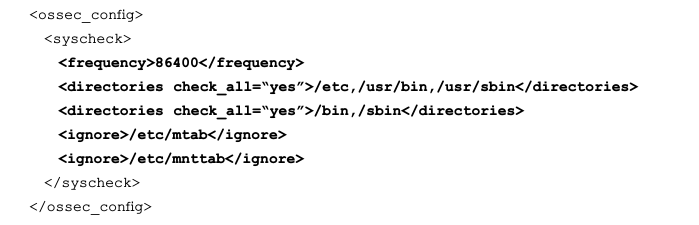
\includegraphics[width=6in,height=3in,keepaspectratio=true]{syscheck.png}}
	\caption{Cấu hình kiểm tra tính toàn vẹn trong ossec.conf}
  \end{figure}
    \item Tạo rules mới nên sử dụng \textless
    if\_group\textgreater syscheck\textless /if\_group\textgreater{} để bao hàm
    group syscheck của OSSEC.
  \end{itemize}
  \subsection{Kiểm tra và phát hiện rootkit}
  \begin{itemize}
    \item OSSEC chỉ có thể kiểm tra rootkit trên hệ điều hành Linux, Unix, và BSD, bên cạnh đó cũng cung cấp khả năng kiểm tra về điều lệ (policy) trên hệ thống Windows, Linux, Unix và BSD.
    \item OSSEC kiểm tra rootkit mức ứng dụng thông qua dấu hiệu và rootkit mức hệ thống thông qua so sánh system call. Ngoài ra còn cung cấp khả năng kiểm tra theo kiểu bất thường (anomaly) để có thể đạt yêu cầu người sử dụng.
    \item Trong mô hình server-agent, việc cấu hình kiểm tra điều lệ (policy) và kiểm tra rootkit được hiện thực trên server và đưa xuống agent.
  \end{itemize}
 \section{Giao diện web OSSEC - OSSEC WUI}
 \subsection{Phần giới thiệu}
 OSSEC HIDS Web User Interface (WUI) cung cấp một giao diện dựa trên web mà thực
 hiện các phân tích thống kê và mối tương quan của dữ liệu thay vì sử dụng các
 thao tác dòng lệnh (command line) để thực hiện.\\\
  Các trang điều khiển chính
 mang lại cho chúng ta một cái nhìn tổng quát vào những gì đang xảy ra khi triển
 khai OSSEC HIDS. Một công cụ tìm kiếm mạnh mẽ có sẵn để theo dõi các sự kiện 
 mà OSSEC HIDS thu thập được và cảnh báo. Tất cả những tập tin bị thay đổi tính
 toàn vẹn được ghi lại, và một giao diện thân thiện cho phép xem các thay đổi
 tập tin theo thời gian. Cuối cùng, một thống kê hữu ích cho phép tổng hợp tất
 cả các sự kiện và cảnh báo được thu thập để cung một cái nhìn thống kê những gì
 đang xảy ra trên mạng của máy tính chúng ta.
 \subsection{Phần cài đặt}
 Các WUI được hỗ trợ trên các hệ điều hành Linux, Unix, và hệ điều hành BSD với
 điều kiện hệ điều hành có khả năng chạy:
 \begin{itemize}
   \item OSSEC HIDS phiên bản 0,9-3 và mới hơn.
   \item Apache HTTP Server là phần mềm để thực hiện HTTP Web Server.
   \item PHP 4.1 và mới hơn:  PHP là một sử dụng rộng rãi, ngôn ngữ general –
   purpose đặc biệt phù hợp để phát triển Web và có thể được nhúng vào HTML.
 \end{itemize}
 \subsection{Thành phần}
Web User Interface có nhiều tab, mỗi trong số đó phục vụ một mục đích, chức năng
cụ thể.
\begin{itemize}
  \item Main: Giao diện điều khiển chính.
  \item Search: Cho phép bạn tìm kiếm thông qua thu thập HIDS OSSEC cảnh báo.
  \item Integrity Checking:  Cho phép bạn tìm kiếm thông qua thu thập từ cảnh
  báo syscheck OSSEC HIDS.
  \item Stats: Hiển thị thống kê về thu OSSEC HIDS cảnh báo.
  \item About:  Hiển thị cấp giấy phép và thông tin bản quyền về các HIDS OSSEC
  và các WUI.
\end{itemize}
\begin{figure}[h!]
	\centering 
	\fbox{
\includegraphics[width=6in,height=3in,keepaspectratio=true]{WUInav.jpg}}
	\caption{Thanh công cụ quản lí WUI của OSSEC}
  \end{figure}
  \begin{enumerate}
    \item Main\\
    Main là giao diện chính của WUI cho phép người dùng có thông tin hợp lệ của
    WUI để xem được những thông tin diễn ra trong việc triển khai OSSEC HIDS.
    Gồm có ba phần chi tiết với nhiệm vụ cụ thể là: Available agents, Latest
    modified files, Latest events.
    \begin{itemize}
      \item Available Agents\\
      Tất cả các cấu hình được hiển thị có sẵn trên tab Main. Các tên agent và địa chỉ IP liên kết được hiển thị cho từng agent. Nếu agent không hoạt động hoặc không thể kết nối đến máy chủ OSSEC HIDS, inactive được hiển thị bên cạnh tên agent.
Nhấp chuột vào các agent cho bạn thông tin chi tiết hơn về máy tính mà
OSSEC HIDS agent được cài đặt.
	  \begin{figure}[h!]
	\centering 
	\fbox{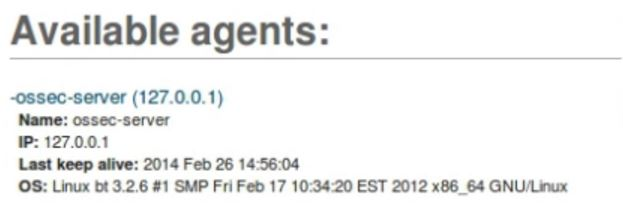
\includegraphics[width=6in,height=3in,keepaspectratio=true]{WUI2.jpg}}
	\caption{Giao diện hiển thị agent hiện có}
  \end{figure}
  \item Latest Modified Files
  \begin{itemize}
    \item Các tập tin mới được sửa đổi (Latest Modified Files) cho thấy một
    danh sách đầy đủ của các tập tin thay đổi mới nhất cho tất cả các agent. Mỗi tập tin sửa đổi được liệt kê theo ngày mà dịch vụ syscheck Báo cáo thay đổi để các máy chủ OSSEC HIDS. Như đã thấy trong hình 7.2, khi bạn nhấn vào tập tin sửa đổi,chi tiết cho các tập tin được hiển thị.
    \item Số lượng các tập tin sửa đổi phụ thuộc vào số lượng agent bạn có cấu
    hình. Điều này được xác định bởi agent\_count + 4 phương trình, agent\_count
    là số lượng agent bạn đã cấu hình. Nếu bạn có 10 agent, nó sẽ chỉ hiển thị
    14 tập tin sửa đổi cuối cùng. Tương tự như vậy, nếu bạn chỉ có một agent, nó
    sẽ chỉ hiển thị năm tập tin sửa đổi cuối cùng. Phương trình agent\_count + 4
    được đặt ra để đảm bảo rằng các giao diện người dùng vẫn duy trì cấu trúc như agent thêm vào được cấu hình.
    \end{itemize}
    \item Latest Events\\
    The Latest events đưa ra các sự kiện mới nhất mà được báo cáo bởi OSSEC HIDS
    agents cho OSSEC HIDS server. Bao gồm một số thông tin cơ bản như: Thời
    gian, chỉ số rule, cấp độ, địa chỉ IP agent, miêu tả, \ldots
   \end{itemize}
   \item Search\\
   Các WUI cung cấp một công cụ tìm kiếm cho phép bạn lọc các tiêu chí cụ thể và
   xem kết quả tìm kiếm trong thời gian thực hoặc thực hiện các phân tích lịch sử trên dữ liệu sự kiện được lưu trữ. Tab tìm kiếm được chia thành ba phần, mỗi phần có một mục đích cụ thể: Tùy chọn tìm kiếm thông báo (Alert search options), kết quả (results) và danh sách thông báo (Alert list)
   \begin{itemize}
     \item Alert Search Options\\
     Cho phép ta xác định các tiêu chí tìm kiếm cảnh báo mà bạn muốn xem.
     Đồng thời nó còn cho phép chúng ta chọn một ngày và phạm vi thời gian cho các cảnh báo được lưu trữ mà chúng ta cần. Nếu chúng ta muốn xem cảnh báo trong thời gian thực thì ta chọn Real time monitoring và chọn các tiêu chí phù hợp. Một số tiêu chí như:
     \begin{itemize}
       \item Minimum level: Đưa ra mức cảnh báo thấp nhất để lọc. Mặc định là
       tất cả (All) và phạm vi là từ 2 đến 15.
       \item Pattern: Chỉ định một mô hình phù hợp để các cảnh báo được tạo ra.
       Mô hình đơn giản matching và công thức Perl regular có thể được sử dụng.
       \item Srcip: Lọc trên một IP nguồn cụ thể trong thông báo được tạo ra.
       \item Location: Bộ lọc trên một OSSEC HIDS agent cụ thể.
     \end{itemize}
     Khi đã hoàn thành việc cấu hình tiêu chuẩn các tiêu chí của bộ lọc tìm kiếm
     cảnh báo, chúng ta phải bấm nút Tìm kiếm (Search) để lấy hồ sơ cảnh báo.
     \item Results\\
     Phần kết quả cho thấy các kết quả truy vấn thông báo dựa trên các bộ lọc
     thiết lập trong Alert Search Options. Ở phía trên của phần kết quả là tổng
     số cảnh báo tìm thấy phù hợp với tiêu chí tìm kiếm. Thông tin sau đó được
     hiển thị trong ba nhóm riêng biệt cho phép chúng ta xem các phân tích kết quả bởi : Mức độ nghiêm trọng (Severity), Rule và IP nguồn ( Src IP).\\
     Trong mỗi nhóm, chúng ta có thể tùy chọn để hiển thị hoặc ẩn các thông báo
     của các loại được chọn. Nhấp vào liên kết màu đỏ bên cạnh các mục nhập bộ
     lọc và có thể bao gồm các mục khác trong bộ lọc.\\
     Ở dưới phần kết quả là các đường dẫn đến các sự kiện đầu tiên và cuối cùng
     nhìn thấy dựa trên bộ lọc cảnh báo hiện tại. Hai liên kết hiển thị ngày tháng và thời gian đóng dấu cho mỗi sự kiện.
     \item Alert List\\
     Danh sách cảnh báo sẽ hiển thị kết quả tìm kiếm với các bộ lọc được xác
     định trong Alert Search Options và phần Result.
   \end{itemize}
   \item Integrity Checking\\
   Phần kiểm tra tính toàn vẹn cung cấp hai tính năng rất quan trọng của WUI:
   một danh sách các tập tin bị sửa đổi của tất cả các agent, và một phương pháp
   dump toàn bộ syscheck cơ sở dữ liệu cho một agent cụ thể.\\
   \textbf{Latest Modified Files (cho tất cả Agents):}\\ 
Phần tập tin sửa đổi mới nhất cho thấy một danh sách đầy đủ của các tập tin bị
thay đổi mới nhất cho tất cả các agent. Mỗi tập tin sửa đổi được liệt kê theo
ngày mà các dịch vụ syscheck báo thay đổi cho máy chủ OSSEC HIDS.\\
	\textbf{Dump Database}\\
	Kiểm tra tính toàn vẹn cho phép bạn cấu hình một agent, và dump toàn bộ nội
	dung của cơ sở dữ liệu syscheck cho agent đó. Dưới phần Latest Modified Files,
	phần Integrity Checking database cung cấp một danh sách hoàn chỉnh của tất cả
	các tập tin hoặc các khóa registry của Windows mà dịch vụ syscheck đã thông báo
	một sự thay đổi tính toàn vẹn. Một vài thông số như : Tên tập tin, mã hash (MD5 hay SHA-1), kích thước tập tin.
	\item Stats\\
	WUI có một công cụ báo cáo thống kê mạnh mẽ cho phép nhanh chóng hiển thị
của các cảnh báo của bạn OSSEC, thay đổi syscheck, và cảnh báo tường lửa cho bất
kỳ ngày, tháng, hoặc năm. Điều này mang đến khả năng chọn một điểm và hiển thị
các thông báo liên quan được  tạo ra bởi các agent và thu thập bởi máy chủ.\\
    WUI được chia thành ba phần báo cáo chính, mỗi phần cung cấp một tổng hợp
    thu thập cảnh báo khác nhau: giá trị tổng hợp bởi mức độ nghiêm trọng, giá
    trị tổng hợp theo rule, tổng giá trị mỗi giờ.
    \begin{itemize}
      \item Giá trị tổng hợp bởi mức độ nghiêm trọng (Aggregate values by
      severity) cho bạn thấy tổng số các cảnh báo được chia nhỏ bởi mức độ nghiêm trọng của các cảnh báo.
      \item Giá trị tổng hợp theo rule (Aggregate Values by Rule ) cho thấy tổng
      số các cảnh báo được chia nhỏ bởi các rule mà tạo ra các cảnh báo.
      \item Tổng giá trị mỗi giờ (Total Values per Hour) cho thấy tổng số các
      cảnh báo được chia nhỏ theo giờ mà các cảnh báo đã báo cáo với OSSEC HIDS
    \end{itemize}
	\item About\\
	Phần giới thiệu của WUI cung cấp bản quyền và thông tin giấy phép cho WUI và
	các OSSEC HIDS. Giấy phép chỉ ra rằng OSSEC HIDS là phần mềm miễn phí và rằng nó có thể phân phối hoặc sửa đổi theo các điều khoản của GNU General Public License (phiên bản 3). Giấy phép này như được xuất bản bởi Free Software Foundation.
  \end{enumerate}

\chapter{Phân tích và thiết kế hệ thống}
\section{Ý tưởng đề xuất}
Các hệ thống HIDS hiện nay sử dụng cơ chế rules-based, tuy cách này
  có lợi thế về mặt thời gian, nhưng trên thực tế, các kiểu tấn công luôn thay đổi, nên
  hệ thống phát hiện được những cuộc tấn công mà chưa được biết đến là 1 điều
  cần thiết.\\\\ 
Các giải thuật gom cụm được áp dụng cho ra các kết quả khá chính xác về
  việc phân cụm sự kiện mạng, giúp cho việc đánh giá cuộc tấn công mạng có
  thể có hướng tiếp cận mới khá khả quan.\\\\ 
Từ các kết luận trên, nhóm đưa ra ý tưởng như sau: tích hợp chương trình
học máy vào trong hệ thống HIDS, để cải tiến quá trình phát hiện các hành vi
xâm nhập, từ đó nâng cao tính an toàn, tính bảo mật cho hệ thống. 
\section{Cách thiết kế hệ thống}
 \begin{figure}[h!]
	\centering 
	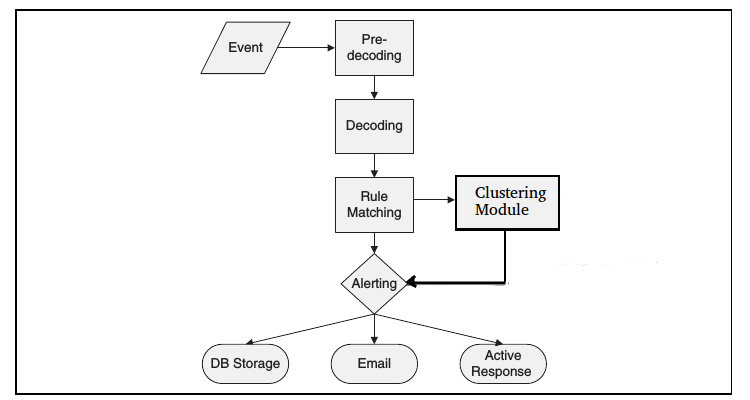
\includegraphics[width=6in,height=3in,keepaspectratio=true]{eventFlowE.png}
	\caption{Cải tiến quá trình phát hiện xâm nhập trong OSSEC}
  \end{figure}
  \subsection{Nhận sự kiện}
  Mỗi khi chương trình trong máy tính hoạt động sẽ tạo ra các log và ghi vào
  trong file log, mỗi 1 log được ghi vào đều là 1 sự kiện. Module này sẽ đảm
  nhiệm việc bắt những đoạn log này cho hệ thống, hệ thống sẽ lấy những đoạn
  log này làm input để thực hiện công việc phát hiện xâm nhập.
  \subsection{Predecode}
   Module này thực hiện nhiệm vụ rút trích các thông tin cơ bản của sự kiện. Các
   thông tin như ngày, giờ, tên chương trình của sự kiện, người dùng thực hiện
   sự kiện đều được rút trích ra, để làm thông tin kiểm tra.\\\\
   Cơ chế rút trích trong module này là sử dụng 1 chuẩn do hệ thống tự định
   nghĩa, các đoạn log của các chương trình khác nhau đều được chuẩn hóa về dạng
   chuẩn này, từ đó hệ thống sẽ rút ra những thông tin cần thiết.
  \subsection{Decode}
   Module này thực hiện nhiệm vụ rút trích các thông tin chính của sự kiện.
   Các thông tin như việc đăng nhập thành công hoặc thất bại các người dùng,
   việc nhập sai mật khẩu, việc chặn gói tin trên ACL, \ldots đều được rút trích
   trong quá trình này.\\\\
   Chúng ta có thể dễ dàng nhận thấy những thông tin trên vô cùng đa dạng. Cấu
   trúc của đoạn log hoàn toàn khác nhau, do vậy việc decode sẽ dễ ra khác nhau
   đối với từng sự kiện, dẫn đến việc mỗi 1 sự kiện đều có 1 decoder riêng.\\\\
   Việc rút trích thông tin trước hết sẽ dự vào tên chương trình mà predecoder
   đã rút trích được, sau đó sẽ tiến hành so sánh lần lượt với các decoder của
   chương trình đó để xác định decoder dùng để rút trích thông tin.\\\\
   Sau khi tiến hành quá trình rút trích, 1 dãy thông tin của
   quá trình predecode và quá trình decode được đưa vào quá trình sau để tiến hành so sánh.
  \subsection{Rule matching}
   Module này thực hiện công việc so sánh các thông tin rút trích được với những
   rule được định nghĩa sẵn trong hệ thống.\\\\
   Quá trình này trước hết sẽ dựa vào decoder được sử dụng để rút trích thông
   tin, tìm ra tất cả các rule của decoder đó. Sau đó tiến hành so sánh lần lượt
   thông tin rút trích được từ sự kiện với từng luật. Do luật trong hệ thống
   được cấu hình theo sơ đồ cây, khi trùng luật ở node cha, hệ thống vẫn tiếp
   tục so sánh với tất cả các luật ở node con. Cảnh báo được phát theo quy
   định của luật cuối cùng được so sánh trùng.\\\\
   Khi so sánh sự kiện với luật sẽ xảy ra 2 trường hợp sau: 
  \begin{enumerate}
    \item Nếu phát hiện trùng: hệ thống sẽ phát ra cảnh báo.
    \item Nếu phát hiện không trùng: dữ liệu rút trích sẽ được đưa vào
    Clustering module.
    \end{enumerate}
   \subsection{Clustering Module}
   Module này sẽ thực hiện công việc kiểm tra lần 2 cho thông tin rút trích
   được, việc kiểm tra này dựa vào học máy.\\\\
   Module sẽ nhận toàn bộ dữ liệu mà hệ thống rút trích được, dựa vào mô hình đã
   được train với tập dữ liệu tốt, gom cụm sự kiện vào 1 trong 2 cụm tấn công
   hoặc bình thường.\\\\
   Việc gom cụm này sẽ dựa vào các thuật toán gom cụm.
   \subsection{Alerting}
   Module này sẽ thực hiện nhiệm vụ phát ra cảnh báo khi phát hiện tấn công,
   được điều khiển bởi Module Rule matching và Module Clustering.
\section{Đánh giá hệ thống}
  Với mô hình trên, nhóm tạo ra hệ thống HIDS kiểu hybrid, kết hợp giữa hệ
thống Rules based và hệ thống Behavior based.\\\\ 
Các dữ liệu rút trích từ sự kiện trước hết phải thông qua
bộ so sánh rule của bản thân OSSEC, nếu sự kiện không trùng mới đi qua hệ
thống Clustering. \\\\
Như vậy, hệ thống mới vẫn giữ được tốc độ của việc phát
hiện xâm nhập trong hệ thống cũ, các dấu hiệu tấn công đã biết vẫn được sử dụng, đảm bảo
việc chính xác trong khi xét các sự kiện đã biết. Bên cạnh đó, các sự kiện không
có dấu hiệu trong rule, được kiểm tra lần 2 trong hệ thống clustering, tăng
thêm tính bảo mật.\\\\  
Ngoài ra, có thể thêm tính năng tự cập nhật rule. Một khi sự kiện được
clustering module phân vào cụm tấn công, và được người dùng xác thực về sự
tấn công đó, hệ thống có thể rút trích các thông tin của sự kiện và viết thành
rule. Sau khi được cập nhật rule, khi gặp lại sự kiện tương tự, hệ thống có thể
nhanh chóng phát hiện tấn công bằng rules.\\\\ 
Clustering module có thể thêm khả năng phân các cuộc tấn công thành nhiều cụm,
chia thành từng loại tấn công, tăng tính rõ ràng cho dữ liệu.
\chapter{Kết luận và hướng phát triển}
Trong quá trình tìm hiểu kiến thức, nhóm nhận thấy có rất nhiều giải thuật học
máy không giám sát trong việc phân cụm dữ liệu. Trong nội dung đề tài thực tập
tốt nghiệp, nhóm đã trình bày nền tảng kiến thức của ba giải thuật gom cụm đơn
giản và phù hợp nhất với nội dụng đề tai của nhóm đó là Kmeans, Mixture of
Gaussian and the EM Algorithm và Self Oraganizing Maps. Bên cạnh đó, nhóm đã tìm
hiểu nền tảng kiến thức của hai giải thuật giúp thu giảm số chiều của ma trận
thuộc tính trước khi áp dụng giải thuật học máy vào ma trận là Principal
Component Analysis và Singular Value Decomposition. Điều này giúp cho việc giảm
thời gian xử lí gom cụm từ ma trận thuộc tính đồng thời còn giúp tăng độ chính
xác.\\\\ 
Sau khi tìm hiểu các kĩ thuật học máy gom cụm và áp dụng vào tập
dữ liệu đầu vào thì nhóm nhận thấy kĩ thuật N-gram và Mixture of 
Gaussian and the EM Algorithm cho kết quả gần với kết quả kì vọng của nhóm nhất mặc dù
chưa có độ chính xác cao.\\\\ 
Nhóm đã thực hiện một mô hình áp dụng mới so
với các công trình liên quan. Nhóm thực hiện chỉ một mô hình học máy giúp thu
giảm thời gian xử lí dữ liệu đầu vào với độ chính xác trong ngưỡng chấp nhận
được. Với OSSEC thì các đề tài trước chỉ xây dựng hệ thống rule cho hệ thống
HIDS, nhóm đưa ra đề xuất đưa các kĩ thuật học máy gom cụm để xây dựng luật
riêng cho OSSED HIDS.\\\\ 
Vì hạn chế về kiến thức mà nhóm chỉ thực hiện
một số chức năng chính có sẵn của công cụ bảo mật OSSEC HIDS mà chưa áp dụng cụ
thể học máy vào để tiến hành phân cụm các cuộc tấn công an ninh mạng.\\\\ 
Hướng phát triển của đề tài khi sang luận văn tốt nghiệp của nhóm là:
\begin{enumerate}
  \item Thực hiện nâng cao hiệu suất và độ chính xác của giải thuật trong việc
  phân cụm tập dữ liệu đầu vào.
  \item Áp dụng các kĩ thuật học máy vào hệ thống mã nguồn mở OSSEC HIDS đồng
  thời kết hợp các chức năng có sẵn để xây dựng một ứng dụng cụ thể có thể phát hiện xâm nhập, tấn công từ bên ngoài.
\end{enumerate}

 
\pagebreak
\begin{thebibliography}{9}  

\bibitem{JohnSOM}
John A. Bullinaria, \emph{Self Organizing Maps: Fundamentals- Introduction to
Neural Networks: Lecture 16}. 2004

\bibitem{KohonenSOM}
Shyam M. Guthikonda, \emph{Kohonen Self-Organizing Maps}. Wittenberg
University. 2005

\bibitem{MehotraMohanRankaSOM}
Mehotra, K., Mohan, C. K., Ranka. S, \emph{Self-Organizing Maps (SOMs)}.
Elements of Artificial Neural Networks. MIT Press. 1997.

\bibitem{SVD} 
Kirk Baker, \emph{Singular Value Deomposition Tutorial}. 2005.

\bibitem{Modeling Syscall}
Eleazar Eskin, Wenke Lee, Salvatore J. Stolfo, \emph{Modeling System Calls
for Intrusion Detection with Dynamic Window Sizes}. DARPA Information
Survivability Conference \& Exposition II, 2001. DISCEX '01. Proceedings. 2001.

\bibitem{Bottou95convergenceproperties}
 Léon Bottou, Yoshua Bengio. \emph{Convergence Properties of the K-Means
 Algorithms}. MIT Press. 1995.
 
 \bibitem{XplaformHIDS}
Gideon Creech. \emph{Developing a high-accuracy cross platform Host-Based
Intrusion Detection System capable of reliably detecting zero-day attacks}. 
2014.

\bibitem{MachineLearningLec}
Andrew Ng. \emph{Lecture Notes – CS229 Machine Learning}. 2012

\bibitem{ossec}
Andrew Hay, Daniel Cid, Rory Bay, \emph{OSSEC Host-Based Intrusion Detection
Guide}. Syngress. 2008

\end{thebibliography}
\end{document}
